\documentclass{bioinfo}
\copyrightyear{2017}
\pubyear{2017}

% amsmath package, useful for mathematical formulas
\usepackage{amsmath}
% amssymb package, useful for mathematical symbols
\usepackage{amssymb}

\usepackage{graphicx}
\usepackage{subfigure}
% cite package, to clean up citations in the main text. Do not remove.
\usepackage{cite}

\usepackage{url}

\begin{document}
\firstpage{1}

% Title must be 150 characters or less
\title[Tracer 1.7]{Posterior summarisation in Bayesian phylogenetics using Tracer 1.7}

\author[Rambaut \textit{et~al.}]{
Andrew Rambaut\,$^{1}$,
Guy Baele$^{2}$,
Dong Xie\,$^{3,4}$,
Alexei J.~Drummond\,$^{3,4}$,
Marc A.~Suchard\,$^{5,6,7}$
}

\address{
$^{1}$Institute of Evolutionary Biology, University of Edinburgh, Edinburgh, UK\\
$^{2}$Department of Microbiology and Immunology, Rega Institute, KU Leuven, Leuven, Belgium\\
$^{3}$Department of Computer Science, University of Auckland, Auckland, NZ\\
$^{4}$Centre for Computational Evolution, University of Auckland, Auckland, NZ\\
$^{5}$Departments of Biomathematics and Human Genetics, David Geffen School of Medicine, University of California, Los Angeles, USA \\
$^{6}$Department of Biostatistics, UCLA Fielding School of Public Health, University of California, Los Angeles, USA \\
$^{7}$Department of Human Genetics, David Geffen School of Medicine at UCLA, University of California, Los Angeles, USA\\
}

\history{Received on XXXXX; revised on XXXXX; accepted on XXXXX}

\editor{Associate Editor: XXXXXXX}

\maketitle


% Please keep the abstract between 250 and 300 words
\begin{abstract}

\section{Motivation:}
Bayesian inference of phylogeny using Markov chain Monte Carlo (MCMC) plays a central role in understanding evolutionary history and processes from molecular sequence data.
Visualising and analysing the samples from the posterior distribution is a key step in any non-trivial Bayesian inference, and it is especially important for methods that employ MCMC.
\section{Results:}
Here we present a software package \emph{Tracer} (version 1.7) for visualising and analysing the trace files generated through Bayesian inference.
The \emph{Tracer} software also provides kernel density estimation, multivariate visualisation, demographic trajectory reconstruction, conditional posterior distribution summary and more.
\section{Availability:}
Tracer is open-source under the GNU lesser general public license and available at \url{http://http://beast.community/tracer} and \url{https://github.com/beast-dev/tracer}.

\section{Contact:}
\href{a.rambaut@ed.ac.uk}{\url{a.rambaut@ed.ac.uk}},
\href{alexei@cs.auckland.ac.nz}{\url{alexei@cs.auckland.ac.nz}}
and
\href{msuchard@ucla.edu}{\url{msuchard@ucla.edu}}

\end{abstract}

\section*{Introduction}

Bayesian inference of phylogeny using Markov chain Monte Carlo (MCMC) \citep{rannala1996probability, mau1999bayesian} flourishes as a popular approach to uncover the evolutionary relationships among operational taxonomic units (OTUs), such as genes, genomes, individuals or species.
MCMC approaches generate samples of model parameter values - including the phylogenetic tree - drawn from their posterior distribution given molecular sequence data and a selection of evolutionary models.
Visualising, tabulating and marginalising these samples is critical for approximating the posterior quantities of interest that one reports as the outcome of a Bayesian phylogenetic analysis.
To facilitate this task, we have developed the Tracer (version 1.7) software package, which allows users to process MCMC log files containing parameter samples and to interactively explore the high-dimensional posterior distribution.
Tracer works automatically with sample output from BEAST 1 \citep{drummond2012bayesian}, BEAST 2 \citep{bouckaert2014beast2}, MrBayes \citep{ronquist2012mrbayes}, RevBayes \citep{hohna2016revbayes}, LAMARC \citep{kuhner2006lamarc}, Migrate \citep{beerli2006comparison} and possibly other MCMC programs from other domains.



\section*{Design and Implementation}

Tracer is able to analyse a single MCMC log and can also combine posterior samples from multiple trace files stemming from an independent evaluation of the same dataset with an identical model combination.
For each trace file loaded, Tracer analyses the posterior samples from all the available parameters, regardless of whether these are discrete or continuous, and present statistical summaries as well as visualisation options for all of these parameters.
Importantly, the effective sample size (ESS) - an important measurement designed for a sampled parameter having continuous values - is immediately apparent in the default view of Tracer and allows users to assess the number of effectively independent draws from the posterior distribution for that parameter (see Figure \ref{fig:overview}:a).
Colour coding is provided for the ESS values to assist the user in determining potential mixing problems in the Bayesian inference performed, with cut-off values at 100 and 200.

Tracer is able to handle three trace types, also known as variable types \citep{mendenhall2012introduction}: real, integer, and categorical.
The real trace type is used to handle quantitative continuous variables, which commonly appear in phylodynamic analyses, whereas the integer trace type allows to deal with quantitative discrete variables and the categorical trace is meant for qualitative categorical variables.
The three trace types are automatically assigned when the trace file is imported but can also manually be set.

Multiple parameter traces can be selected from the traces panel, which will result in a side-by-side comparison or overlay of the selected parameters' visualisations for the different traces (see Figure \ref{fig:overview}:b-e).
Multiple trace files can be selected in a similar fashion to compare posterior samples between different replicates of an analysis.
If multiple trace files have the same file name,  then a ``Combined'' trace will automatically appear, which can be selected as well as the individual trace files.
Tracer consists of four panels that allow to present both individual and joint visualisation options for either a single or multiple selected trace files:

\begin{itemize}

\item Estimates: this panel reports common summary statistics such as the mean, standard deviation, highest posterior density interval, ESS, and other statistics concerning the selected parameter(s).
A histogram presenting the frequency distribution over values will be shown for a single selected parameter of any trace type (see Figure \ref{fig:overview}:a), whereas side-by-side boxplots will be shown when multiple continuous parameters are selected (see Figure \ref{fig:overview}:b).

\item Marginal Density: this panel shows a density plot for the posterior sample of the selected parameter(s). Kernel density estimation (see Figure \ref{fig:overview}:c), histograms and violin plots (see Figure \ref{fig:overview}:d) are available for continuous traces, whereas frequency plots are employed for integer traces.

\item Joint-Marginal: visualisation in this panel only appears when two or more parameters are selected. The actual visualisation depends on the trace type of the selected parameters. We show several examples in the next section of the paper.

\item Trace: this panel shows a line plot connecting the posterior samples of one or more selected parameters against state or generation number (see Figure \ref{fig:overview}:e). Such a trace plot is typically used to assess mixing, select a suitable burn-in and identify trends that suggest convergence issues.

\end{itemize}


Tracer offers an elegant solution of visualising conditional posterior distributions.
A typical use case involves support for Bayesian stochastic search variable selection (BSSVS), a form of model averaging, in which parameters appear in the likelihood function only when a specific model is indicated by an indicator function.
When BSSVS is used, the posterior distribution of the parameter should not include those states that were sampled from the prior when its model was not part of the likelihood.
Discrete phylogeographic analyses frequently employ such an approach due to the potentially large amount of transition rates that need to be estimated \citep{Lemey2009}, but this is also relevant when employing model averaging approaches such as for relaxed molecular clocks for example \citep{Li2012}.

Additionally, Tracer provides demographic reconstruction resulting in a graphical plot, often applied to reconstruct epidemic dynamics.
Depending on the actual demographic model used in the analysis, an additional file containing samples from the posterior tree distribution will be required.
The currently available models are constant size, exponential and logistic growth \citep{drummond2002estimating}, Bayesian coalescent skyline \citep{drummond2005bayesian}, Gaussian Markov Random Field (GMRF) Bayesian skyride \citep{minin2008smooth}, and Bayesian coalescent skygrid \citep{gill2012improving}.
%Not sure if the statement below is correct ...
All of these demographic models are available in BEAST 1 \citep{drummond2012bayesian} and BEAST 2 \citep{bouckaert2014beast2}.
%Besides these, ``Lineages Through Time'' (?) is also available to plot the quantiles of the number of lineages against time, which describes the change of diversification of all organisms over time. %citation?


\begin{figure}[ht]
\subfigure[Tracer overview]{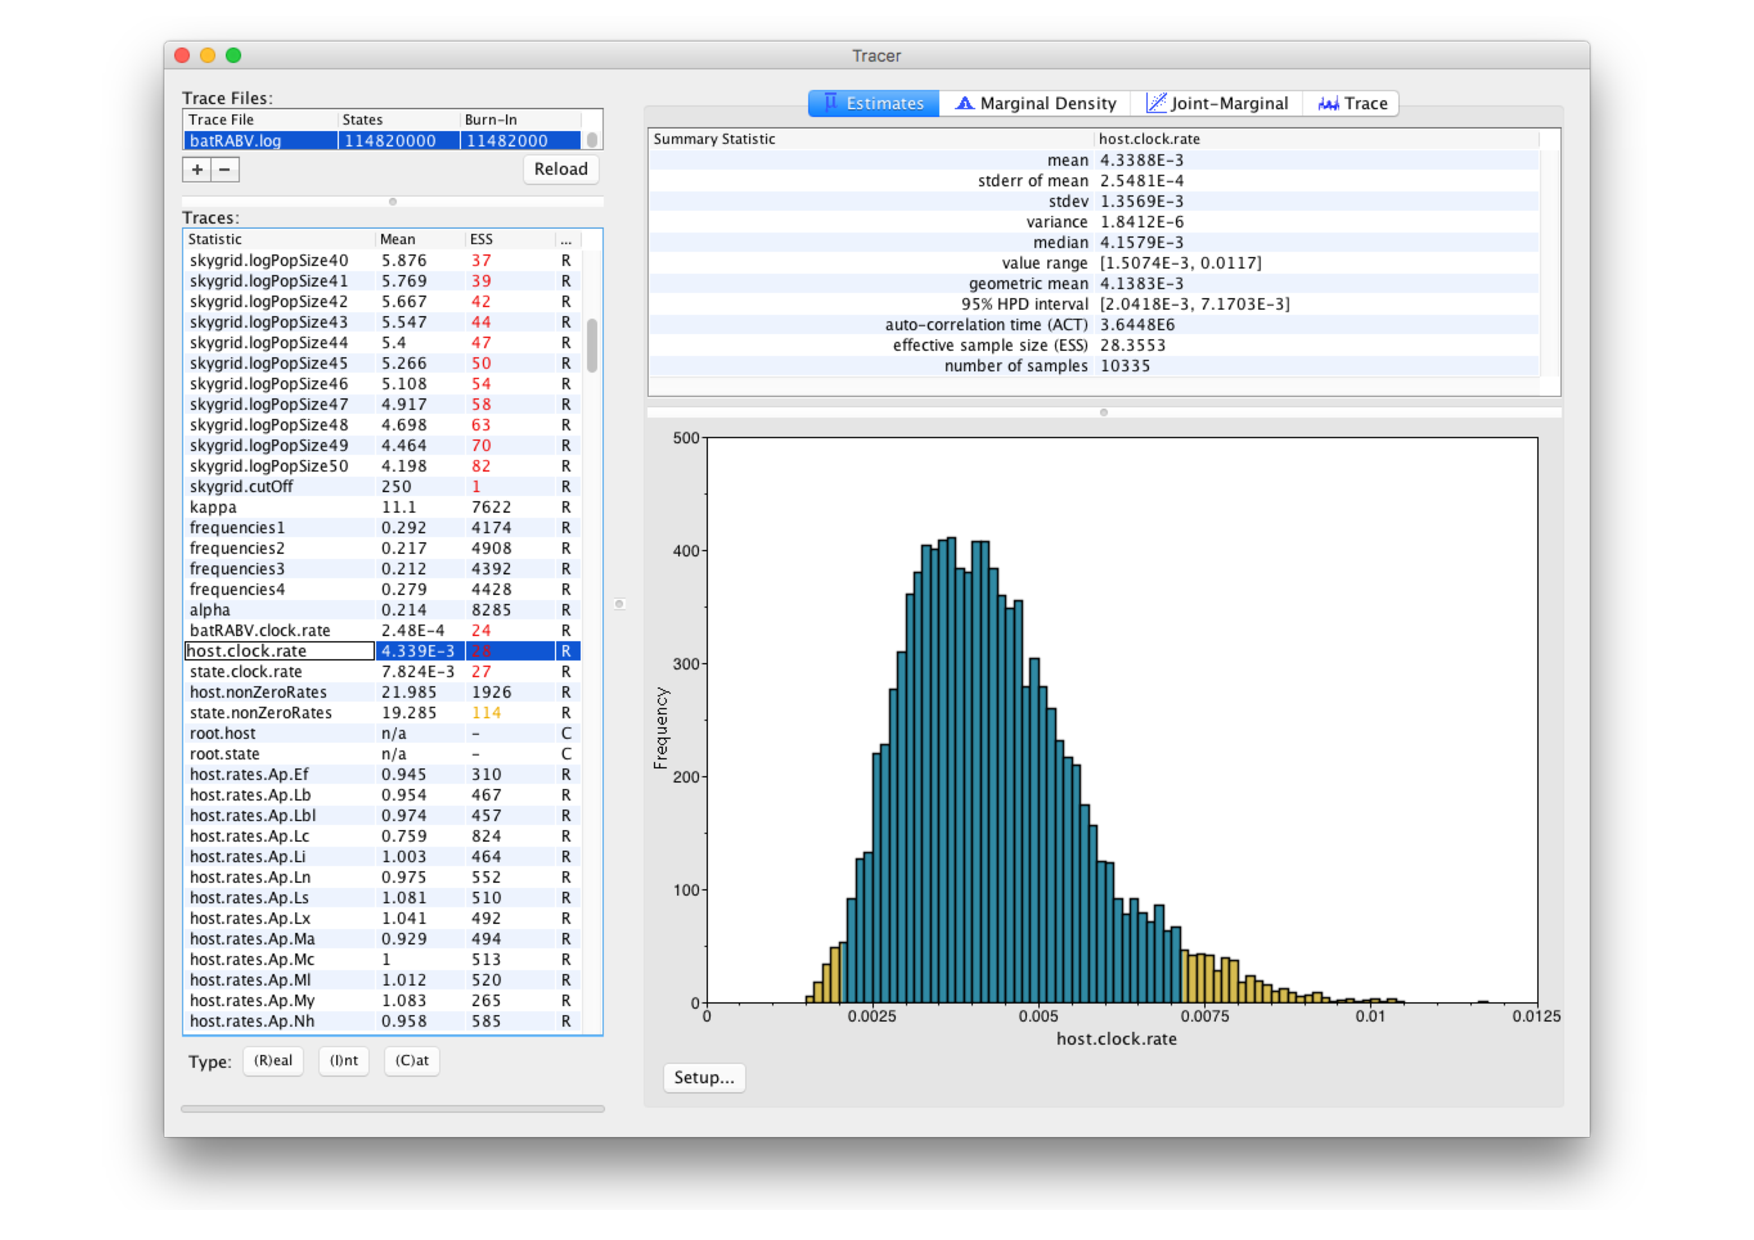
\includegraphics[width=0.47\textwidth]{./figures/rabv-overview.pdf}}
\subfigure[Boxplot]{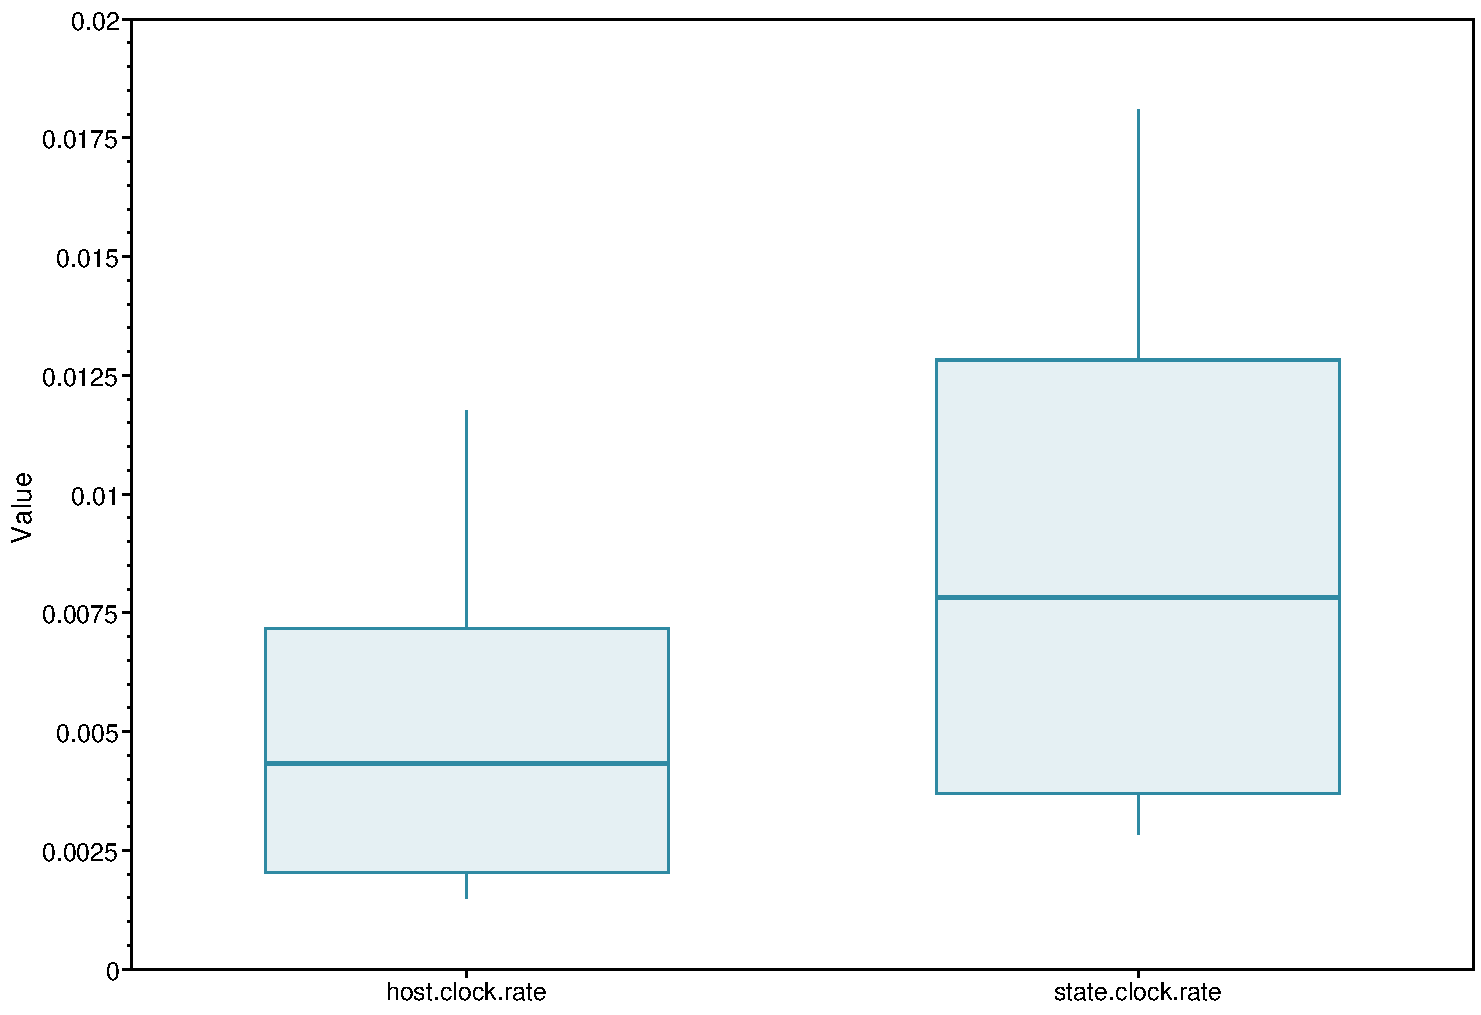
\includegraphics[width = .23\textwidth, height = 3cm]{./figures/rabv-boxplots.pdf}}
\subfigure[Density]{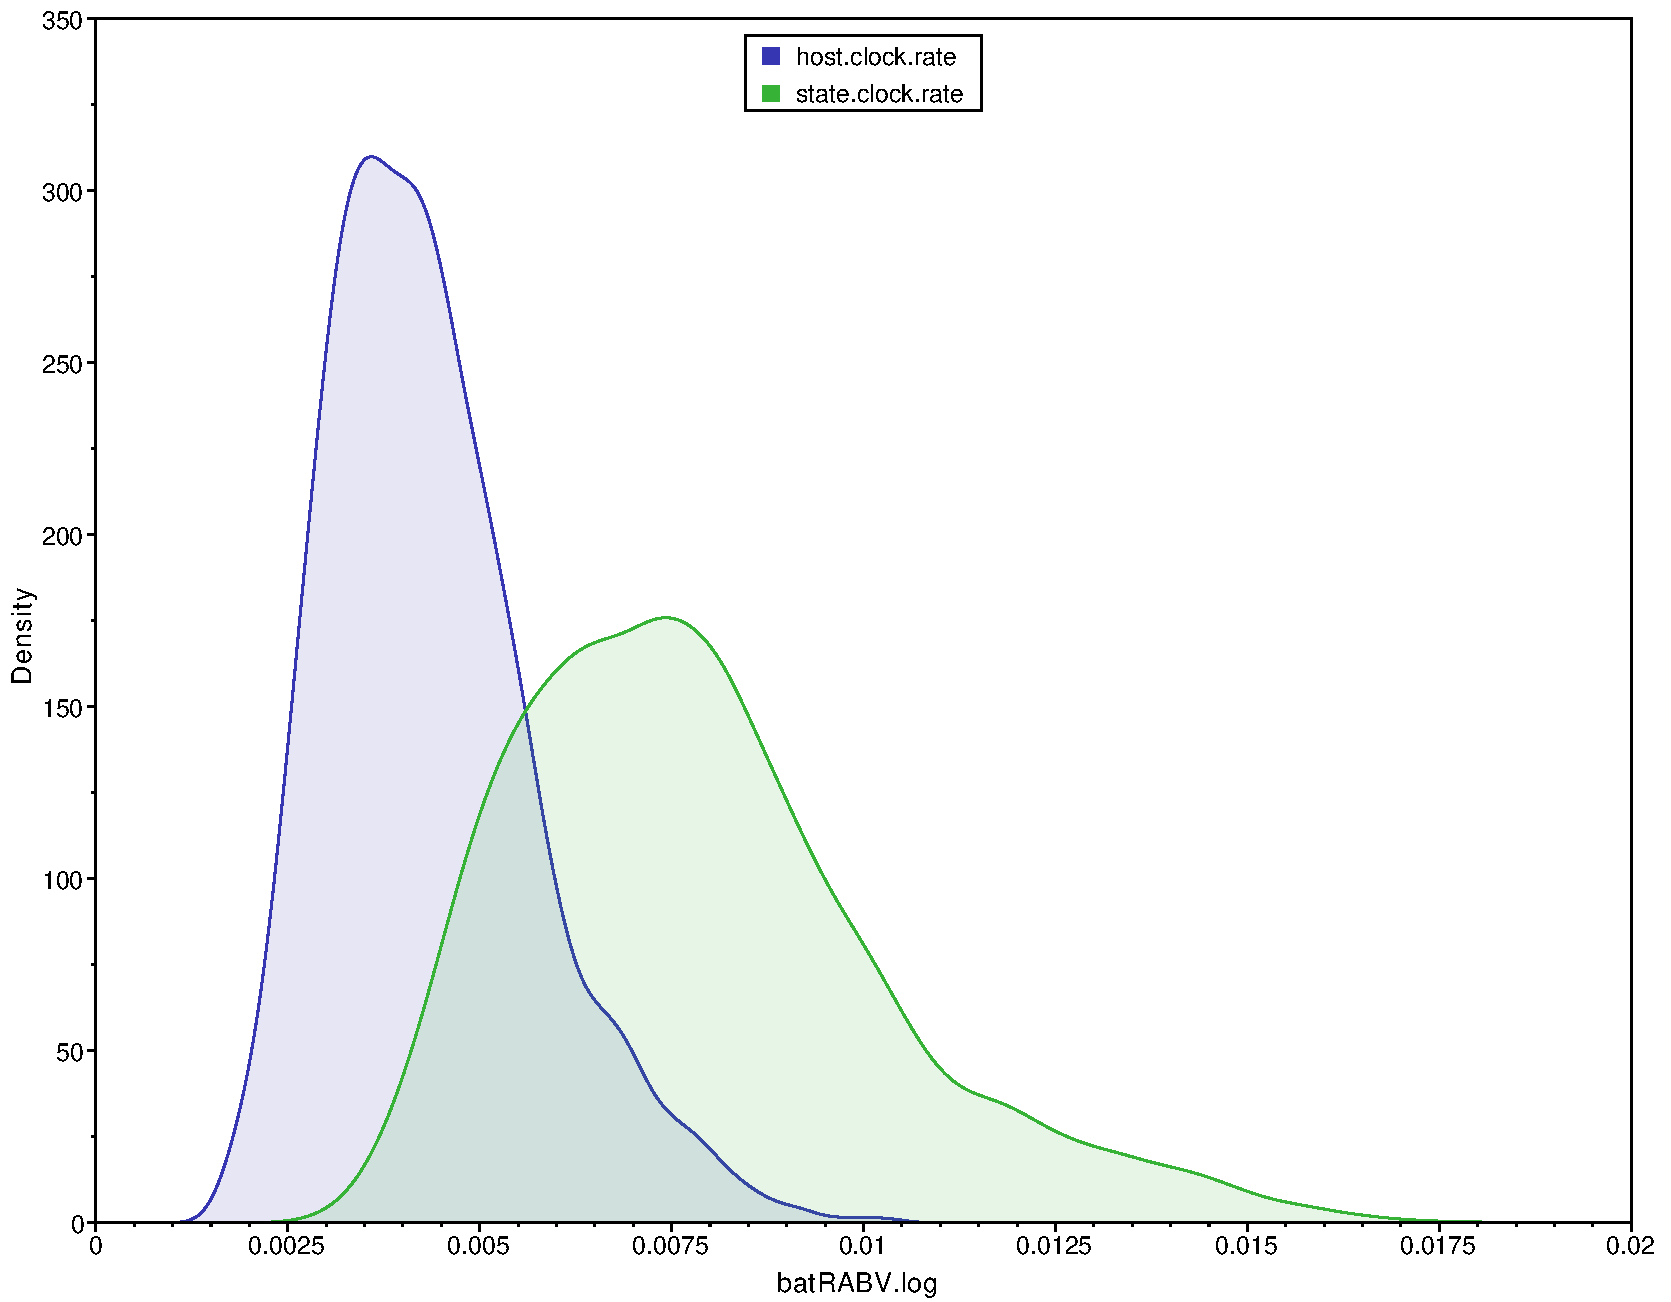
\includegraphics[width = .23\textwidth, height = 3cm]{./figures/rabv-density.pdf}}\\
\subfigure[Violin]{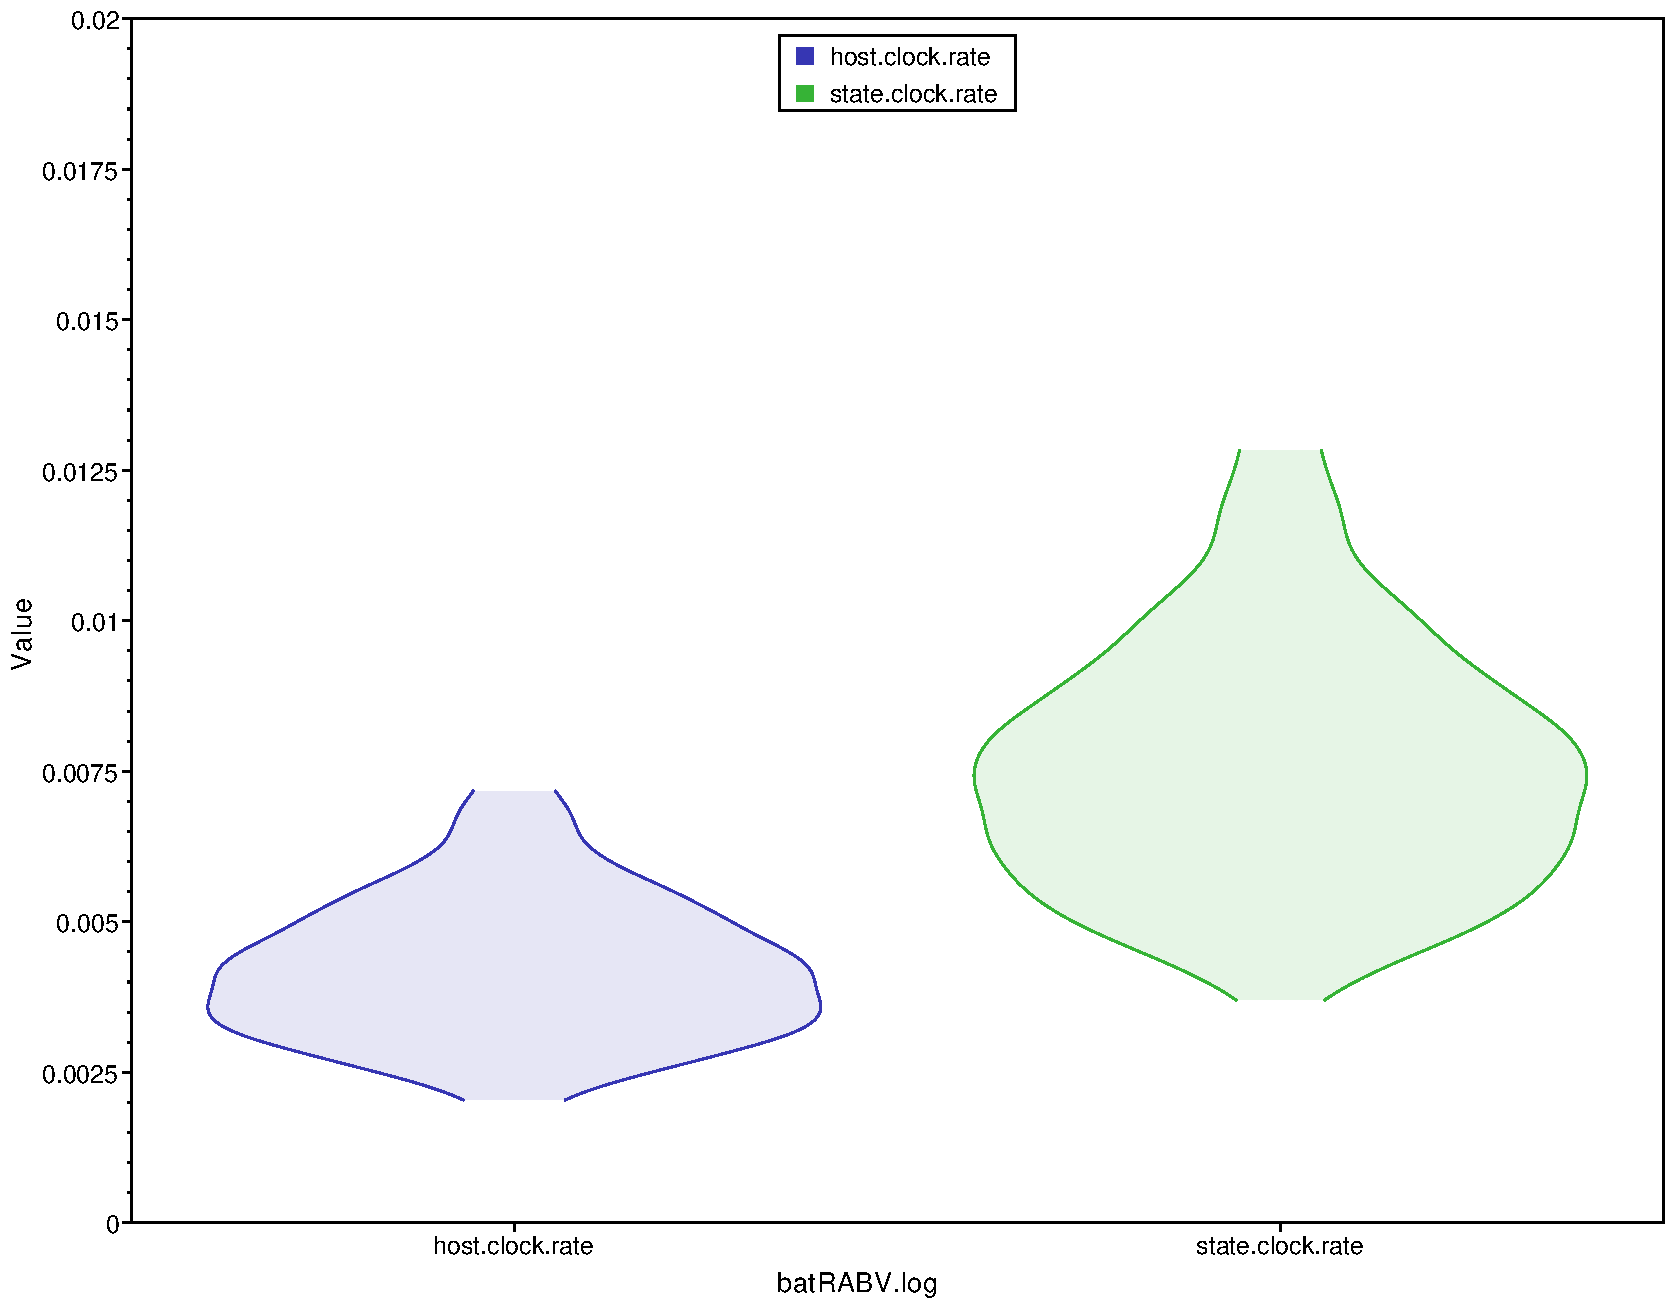
\includegraphics[width = .23\textwidth, height = 3cm]{./figures/rabv-violin.pdf}}
\subfigure[Trace]{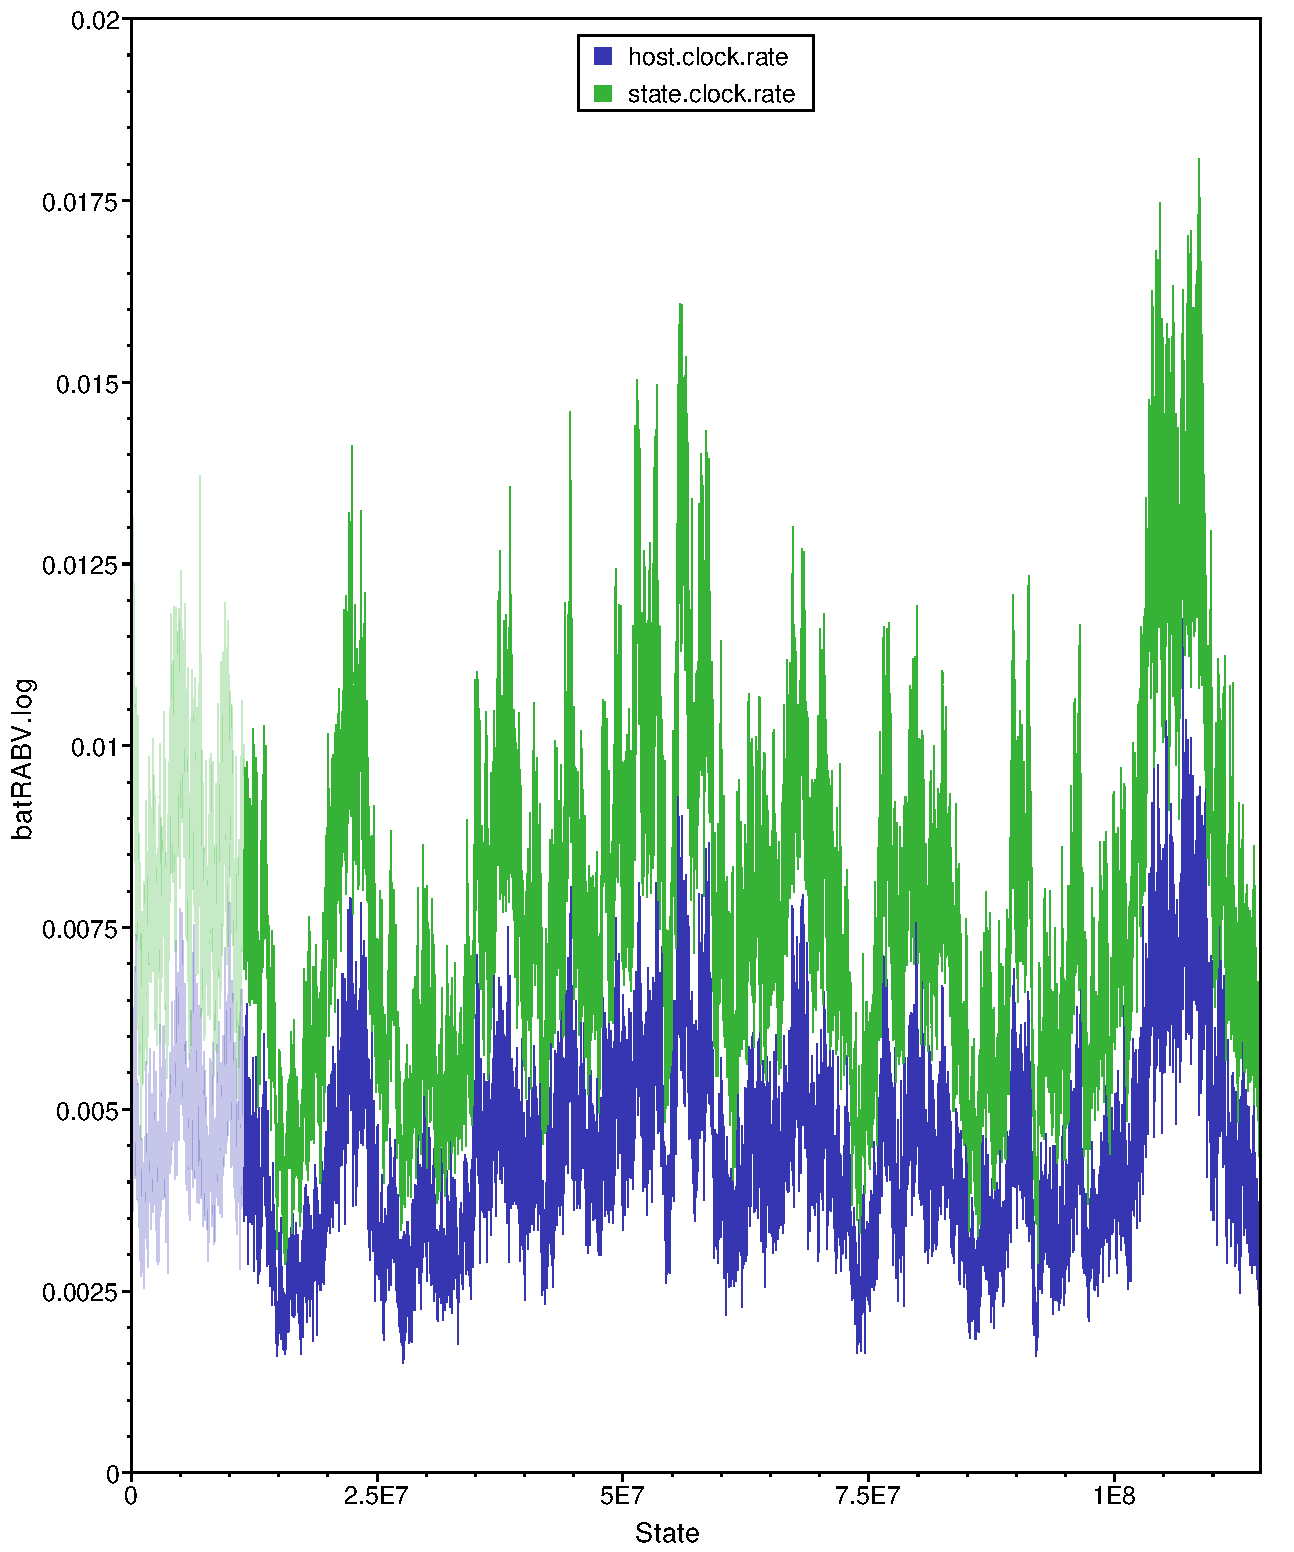
\includegraphics[width = .23\textwidth, height = 3cm]{./figures/rabv-traces.pdf}}
\caption{Overview of Tracer functionality and individual parameter visualisations: (a) Main Tracer panel upon loading a single trace file; (b) boxplot representation of two continuous parameters; (c) kernel density estimates; (d) violin plots; (e) the actual traces connecting the parameter values visited by the Markov chain.}
\label{fig:overview}
\end{figure}



\section*{Example}

\subsection*{Cross-species dynamics of rabies virus in North American bats}

We provide on example on reconstructing the spatial dispersal and cross-species dynamics of rabies virus (RABV) in North American bat populations based on a set of 372 nucleoprotein gene sequences (nucleotide positions: 594-1353).
The data set comprises a total of 17 bat species sampled between 1997 and 2006 across 14 states in the United States \citep{Streicker}, including two additional species that had been excluded from the original analysis owing to a limited amount of available sequences \citep{Faria2013}.
%We also include a viral sequence with an unknown sampling date (accession no. TX5275, sampled in Texas from Lasiurus borealis), which will be adequately accommodated in our inference.
We estimate the ancestral locations of RABV using a Bayesian discrete phylogeographic approach and, at the same time, infer the history of host jumping using the same model approach \citep{Lemey2009}.
We employ the Bayesian skygrid coalescent model \citep{gill2012improving} to estimate the effective population sizes over time.


\begin{figure}[ht]
\subfigure[TangHuLu chart]{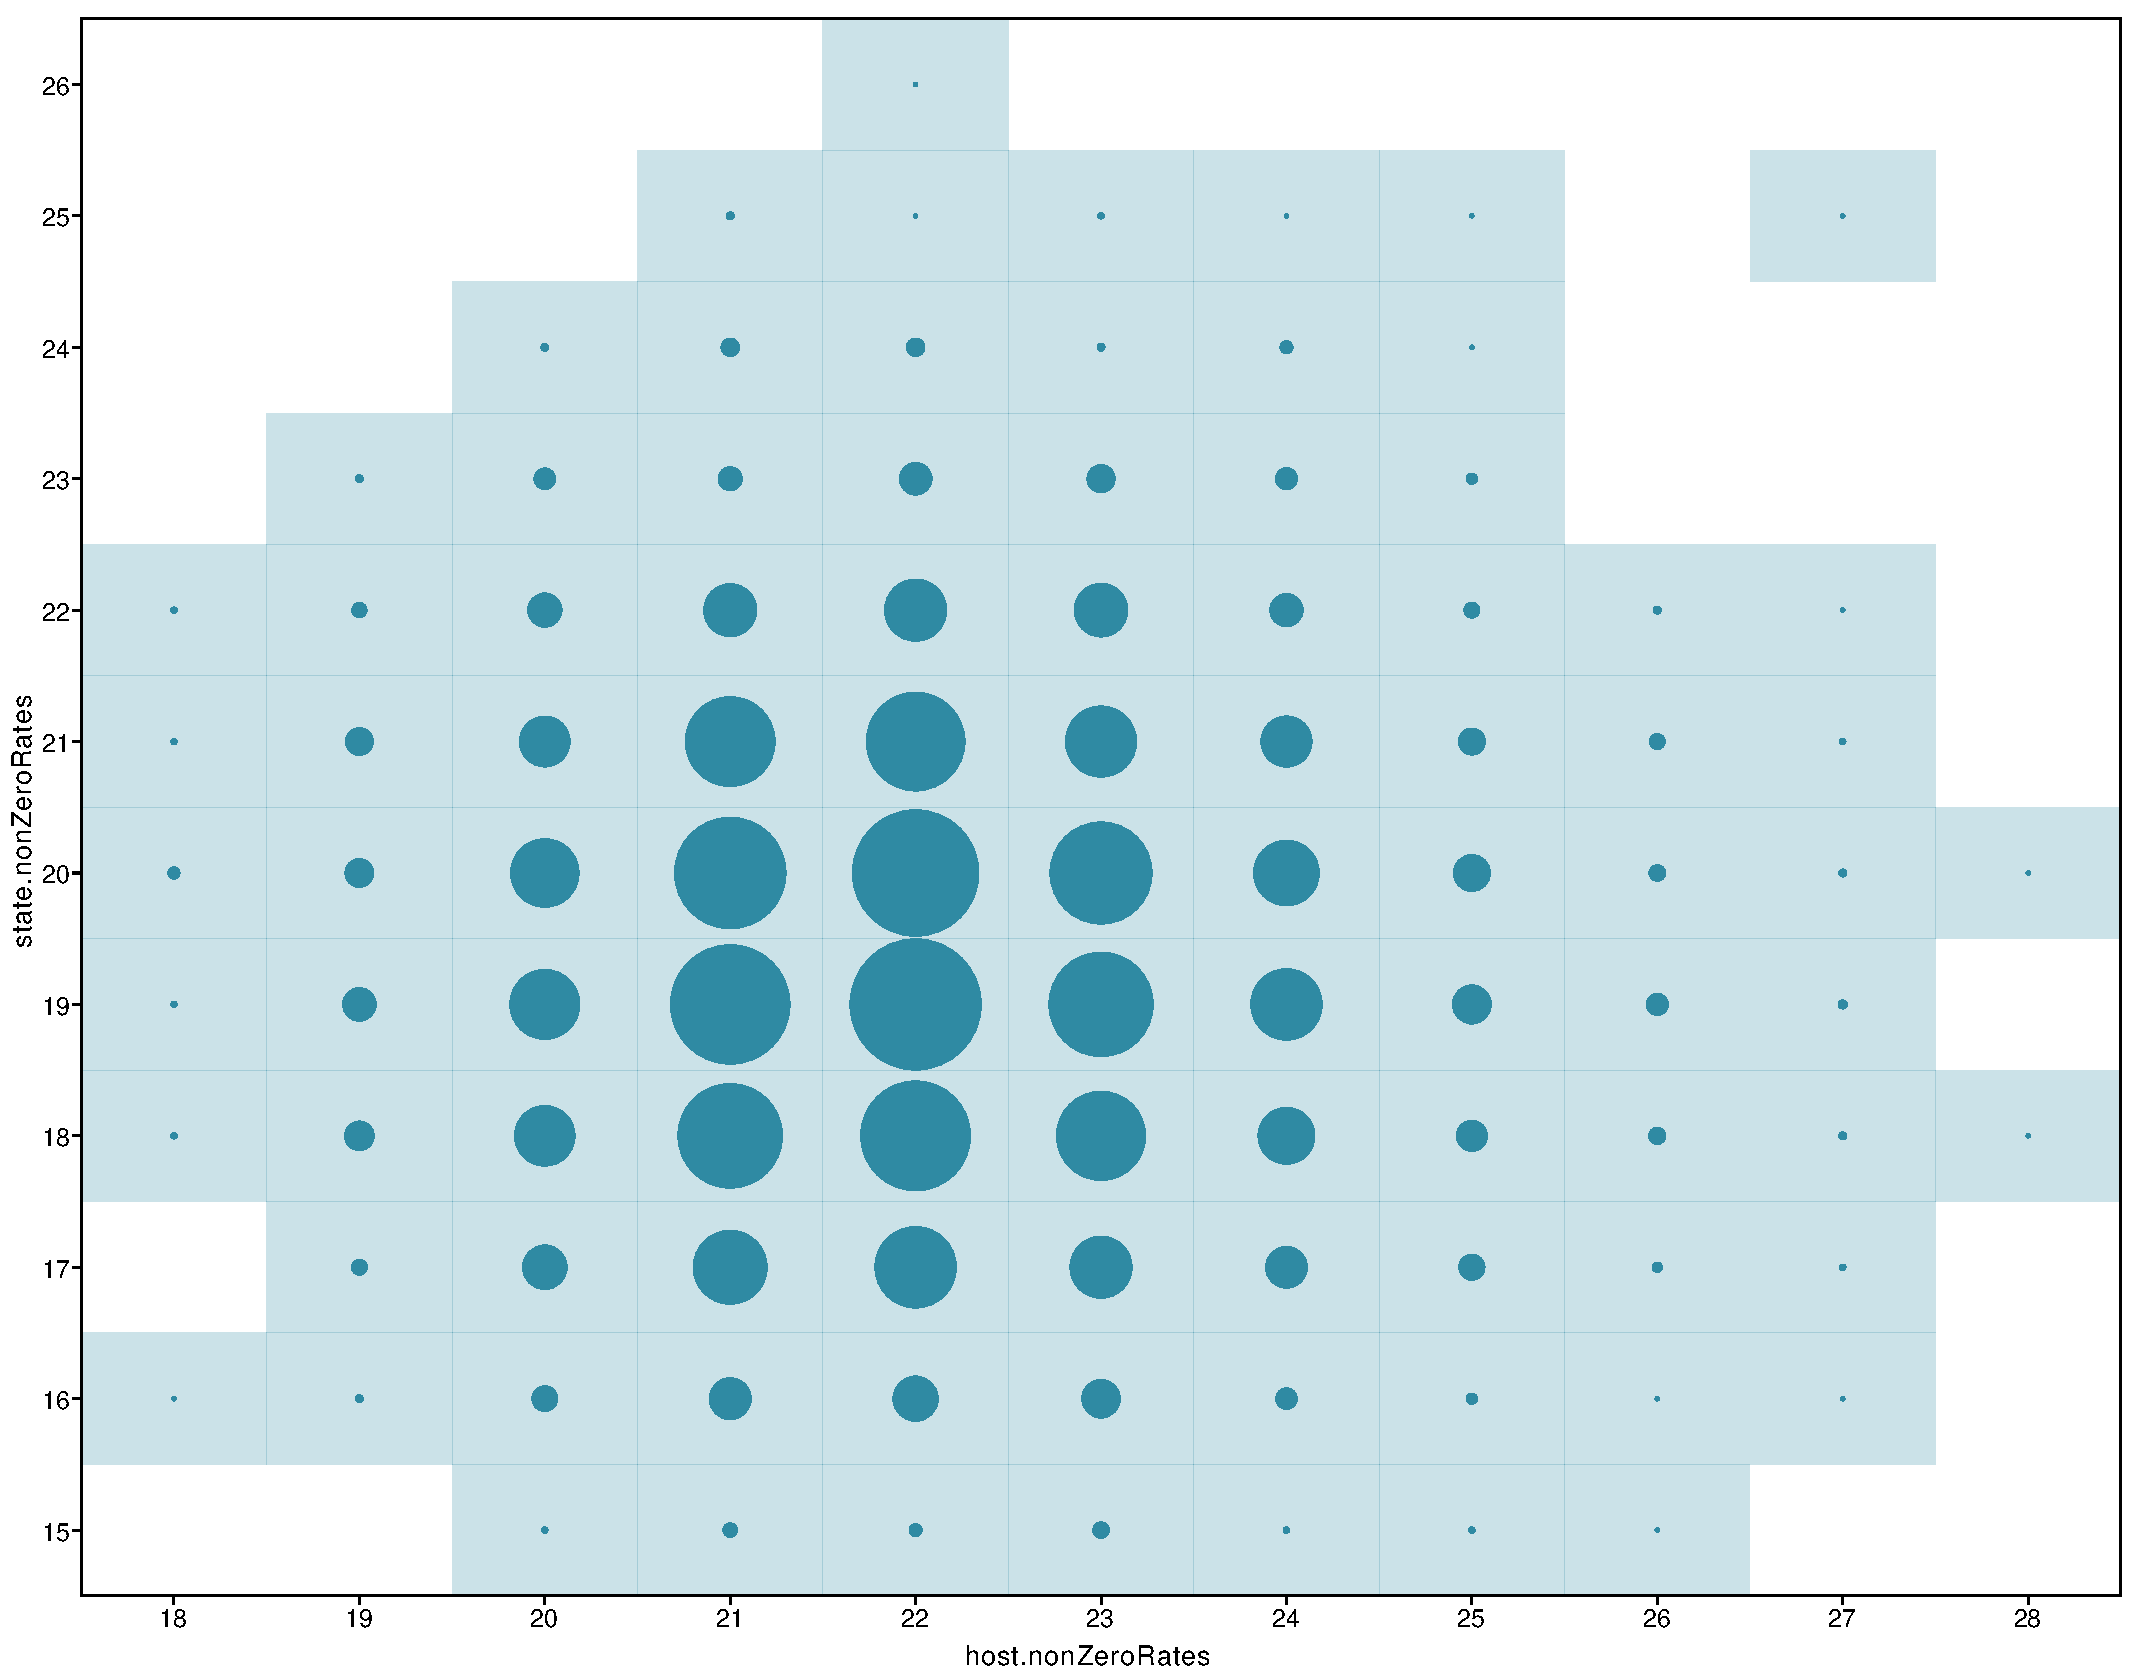
\includegraphics[width = .23\textwidth, height = 3cm]{./figures/rabv-integerjointmarginal.pdf}}
\subfigure[Marginal density]{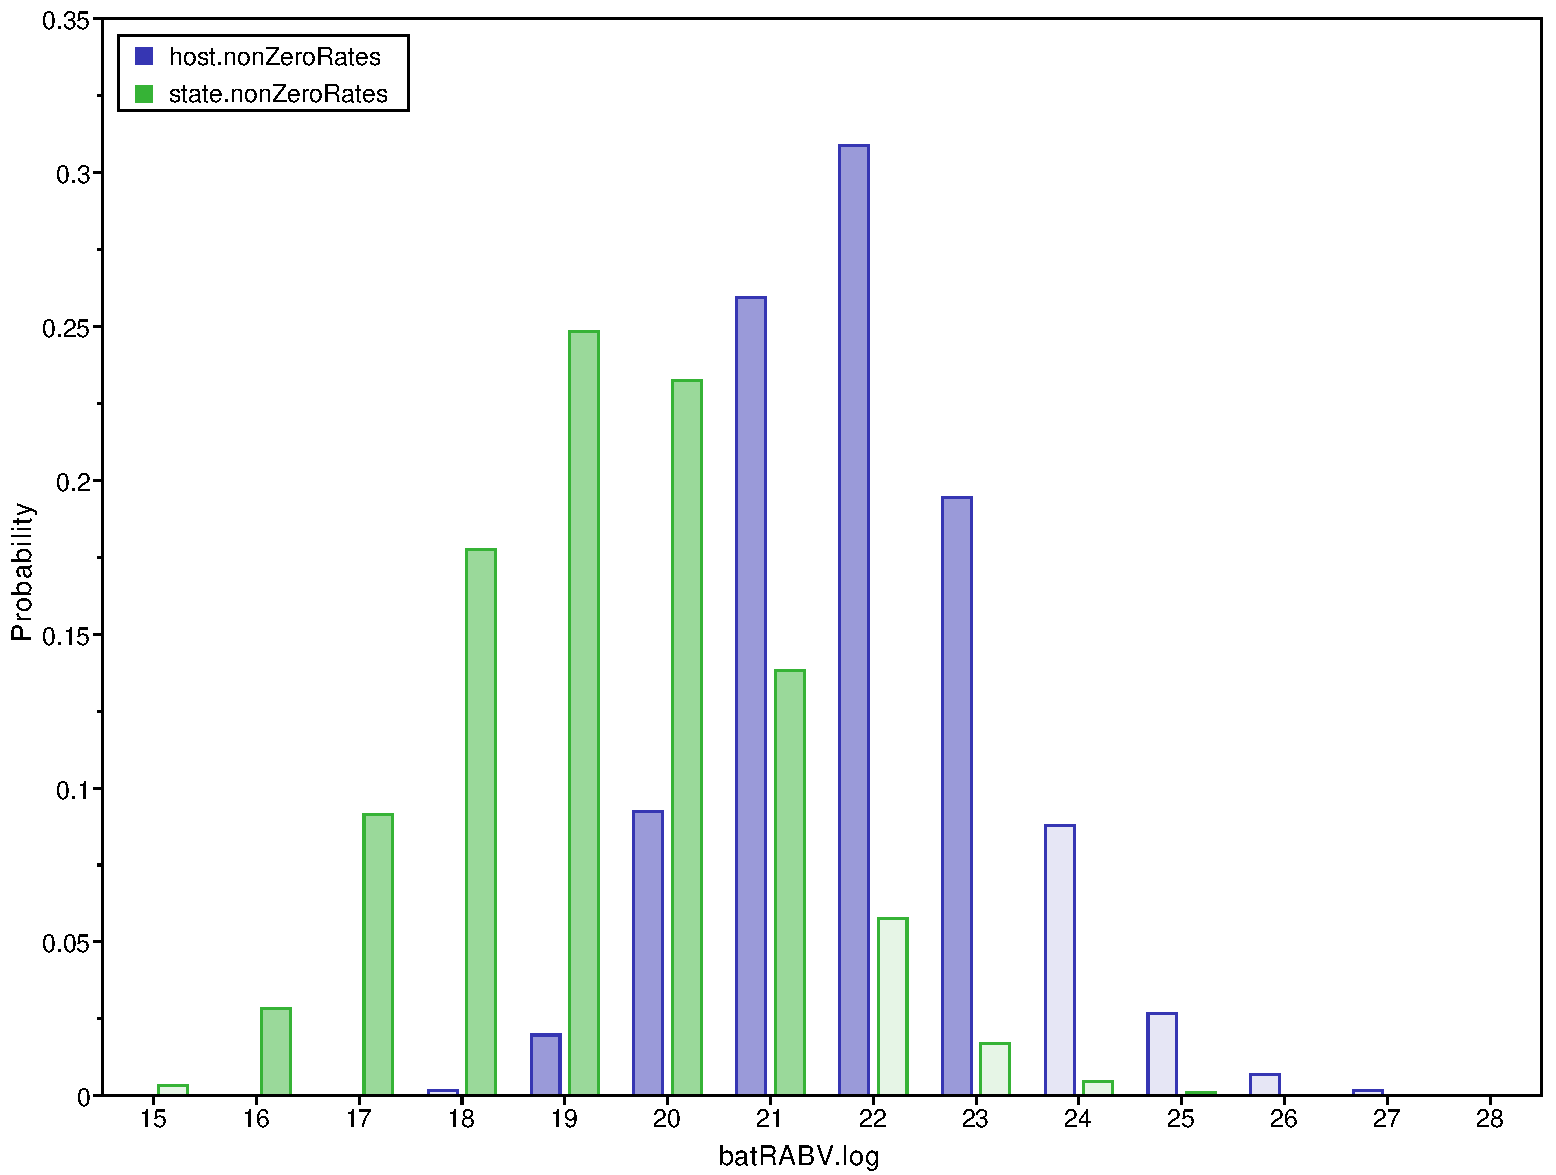
\includegraphics[width = .23\textwidth, height = 3cm]{./figures/rabv-integermarginaldensity.pdf}} \\
\subfigure[Scatter plot]{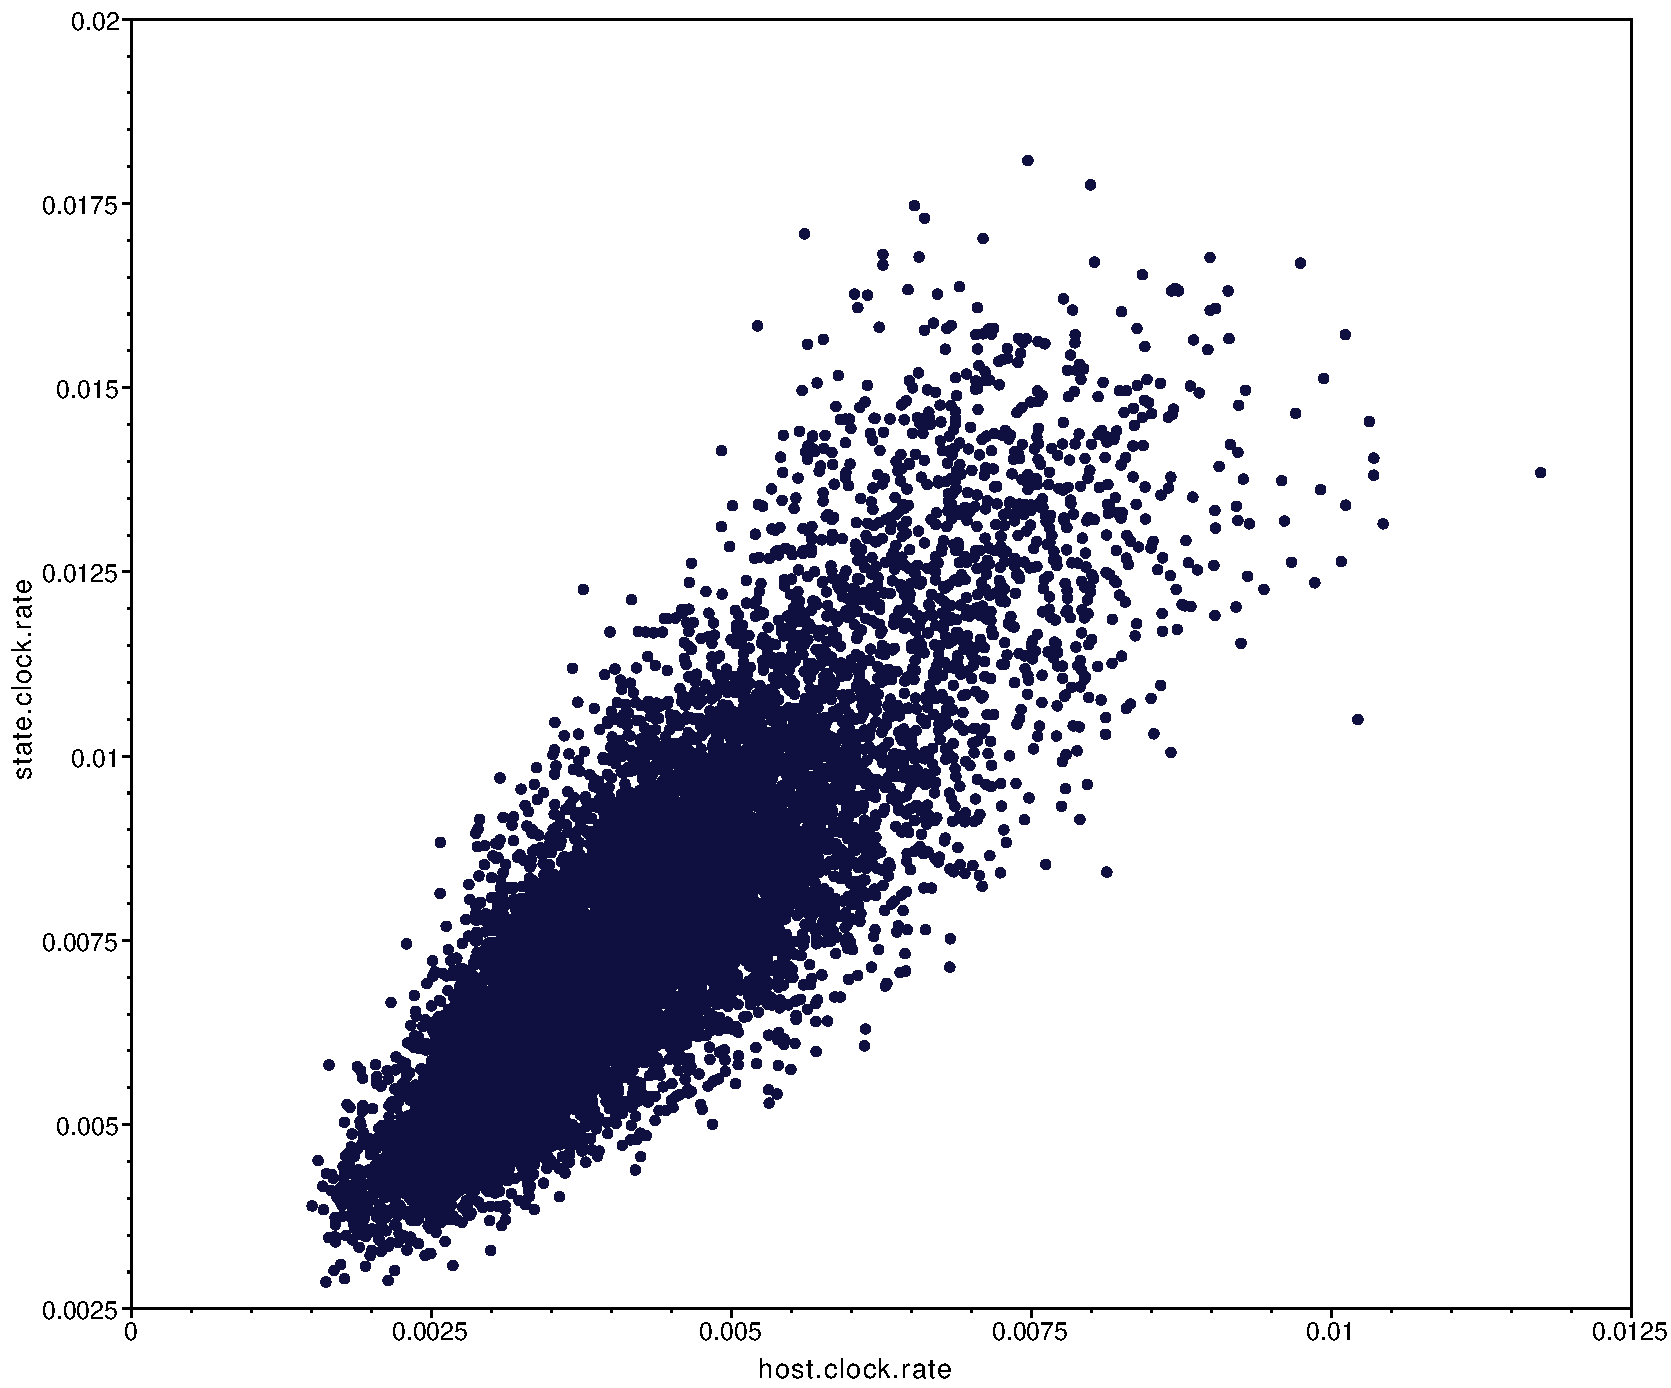
\includegraphics[width = .23\textwidth, height = 3cm]{./figures/rabv-correlation.pdf}}
\subfigure[Correlation plot]{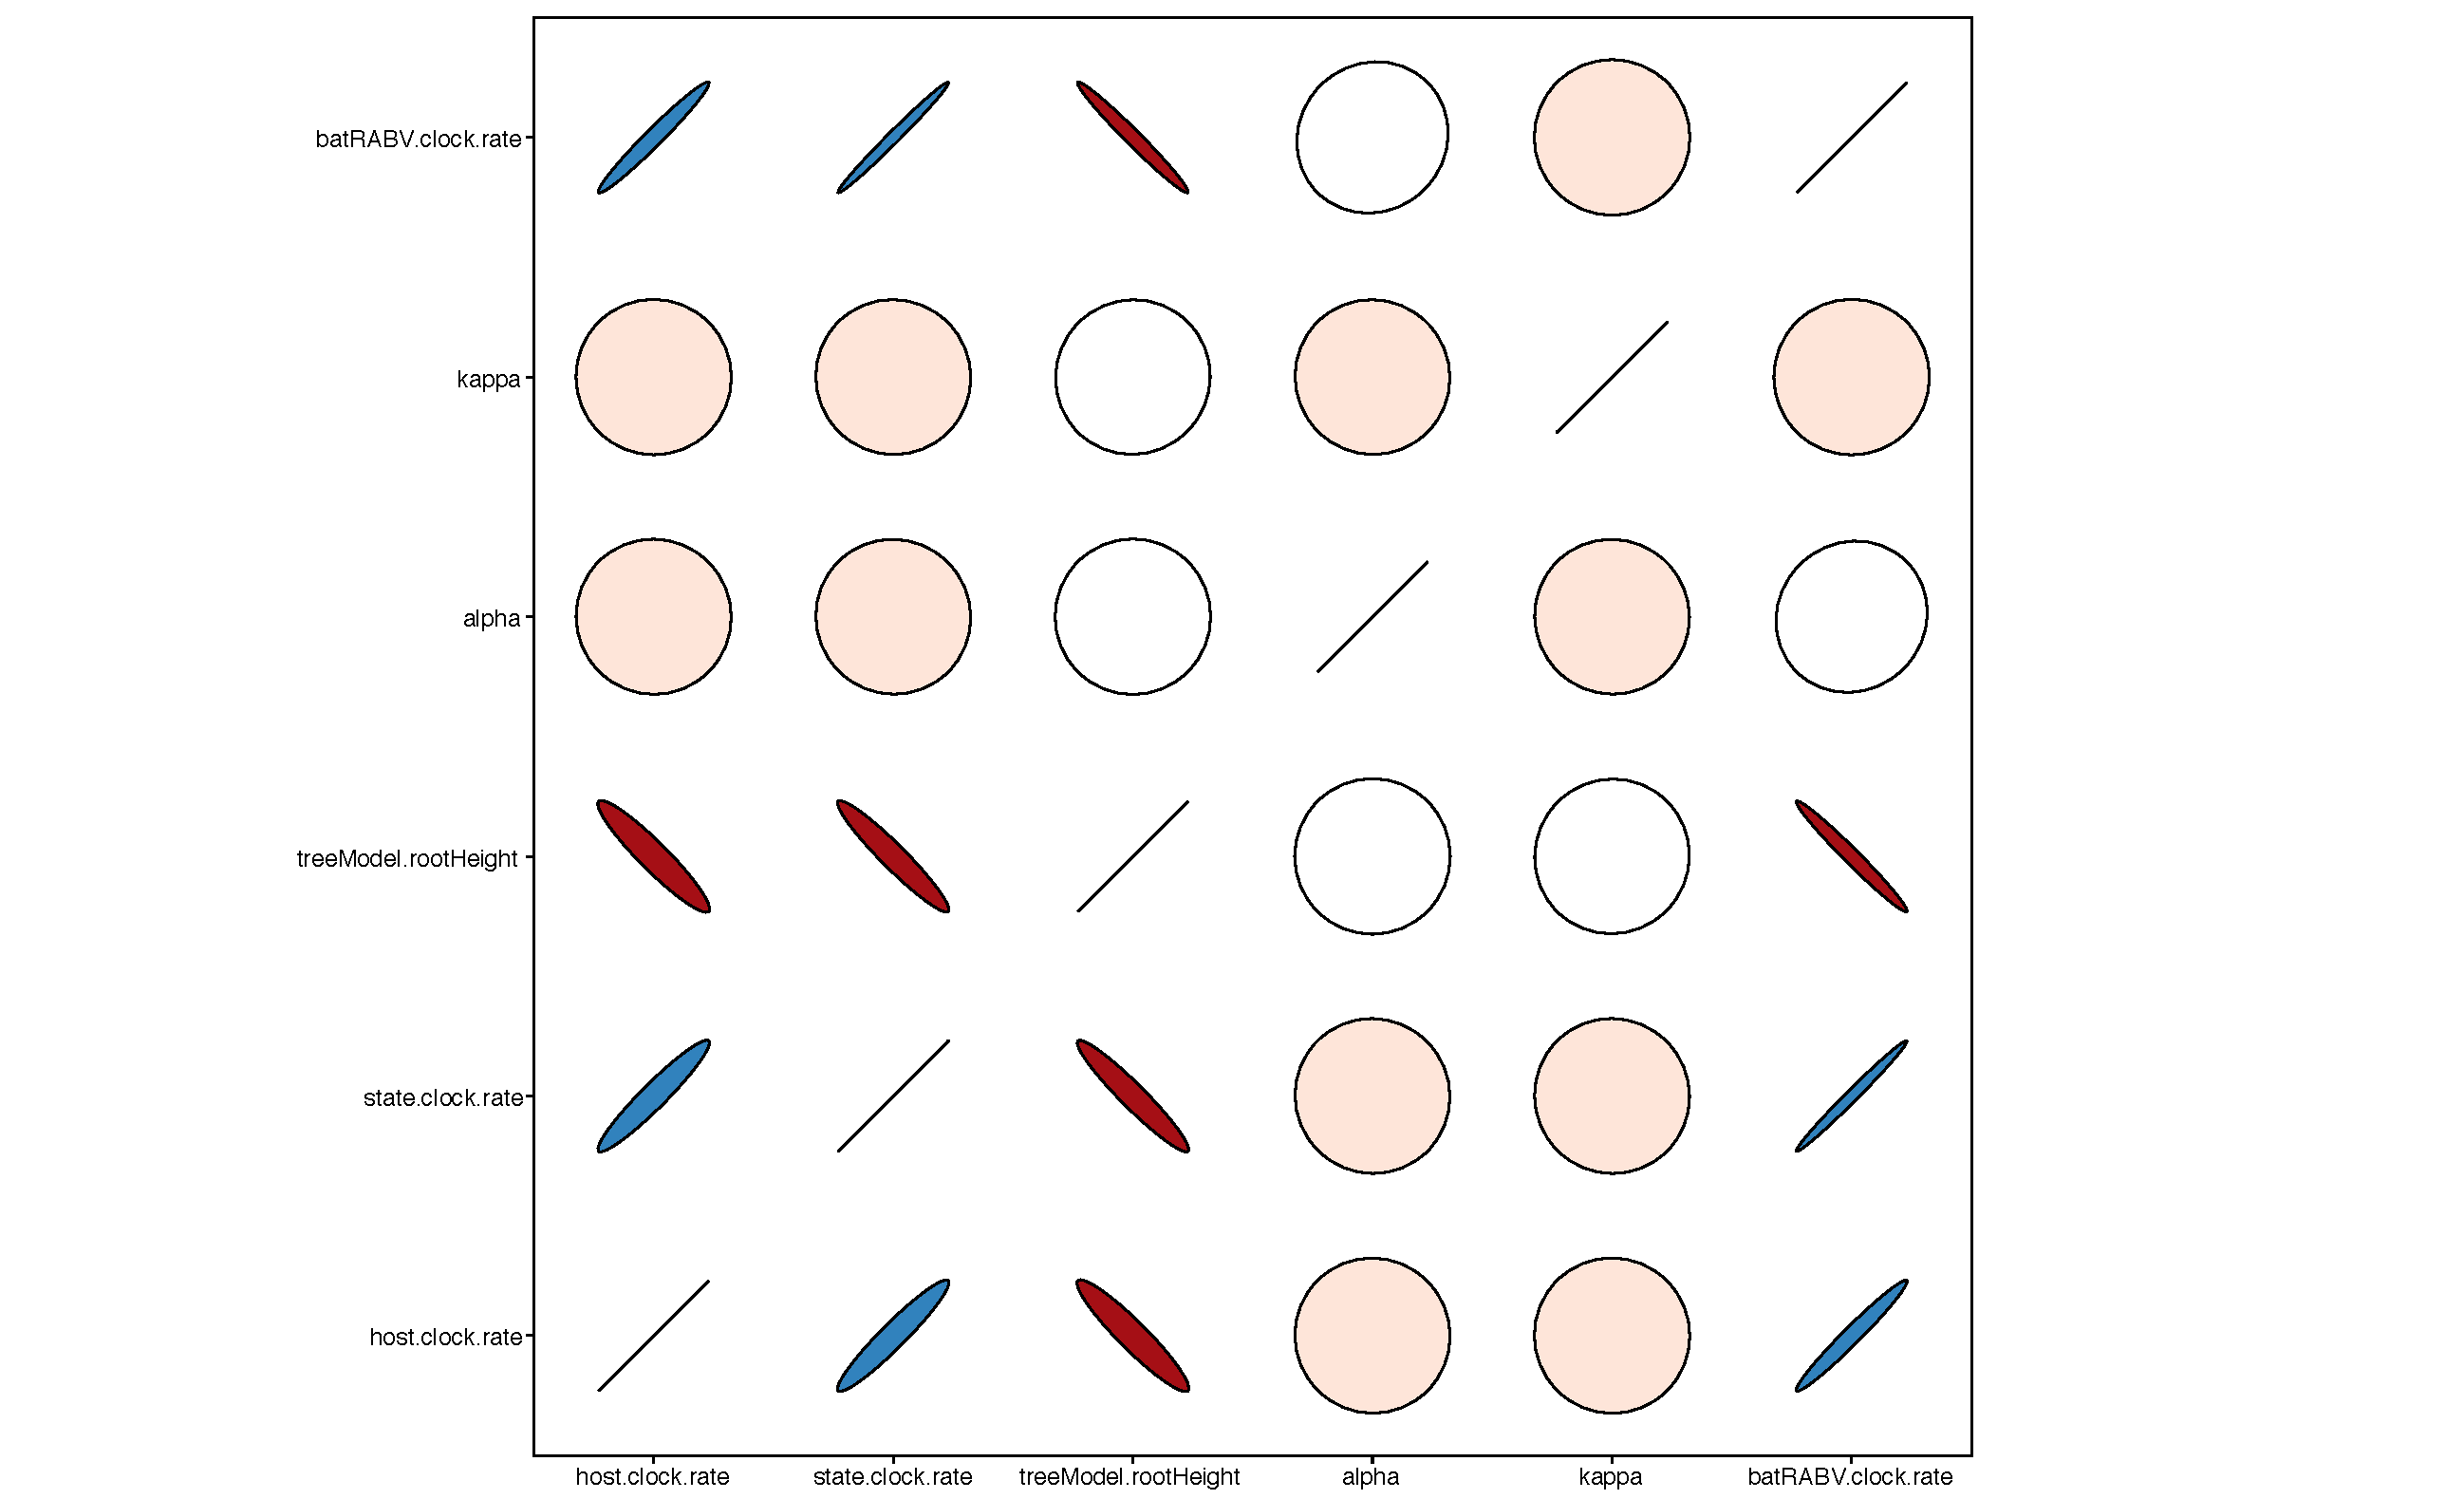
\includegraphics[width = .23\textwidth, height = 3cm]{./figures/rabv-joint-real.pdf}} \\
%\subfigure[Box-and-whisker plot]{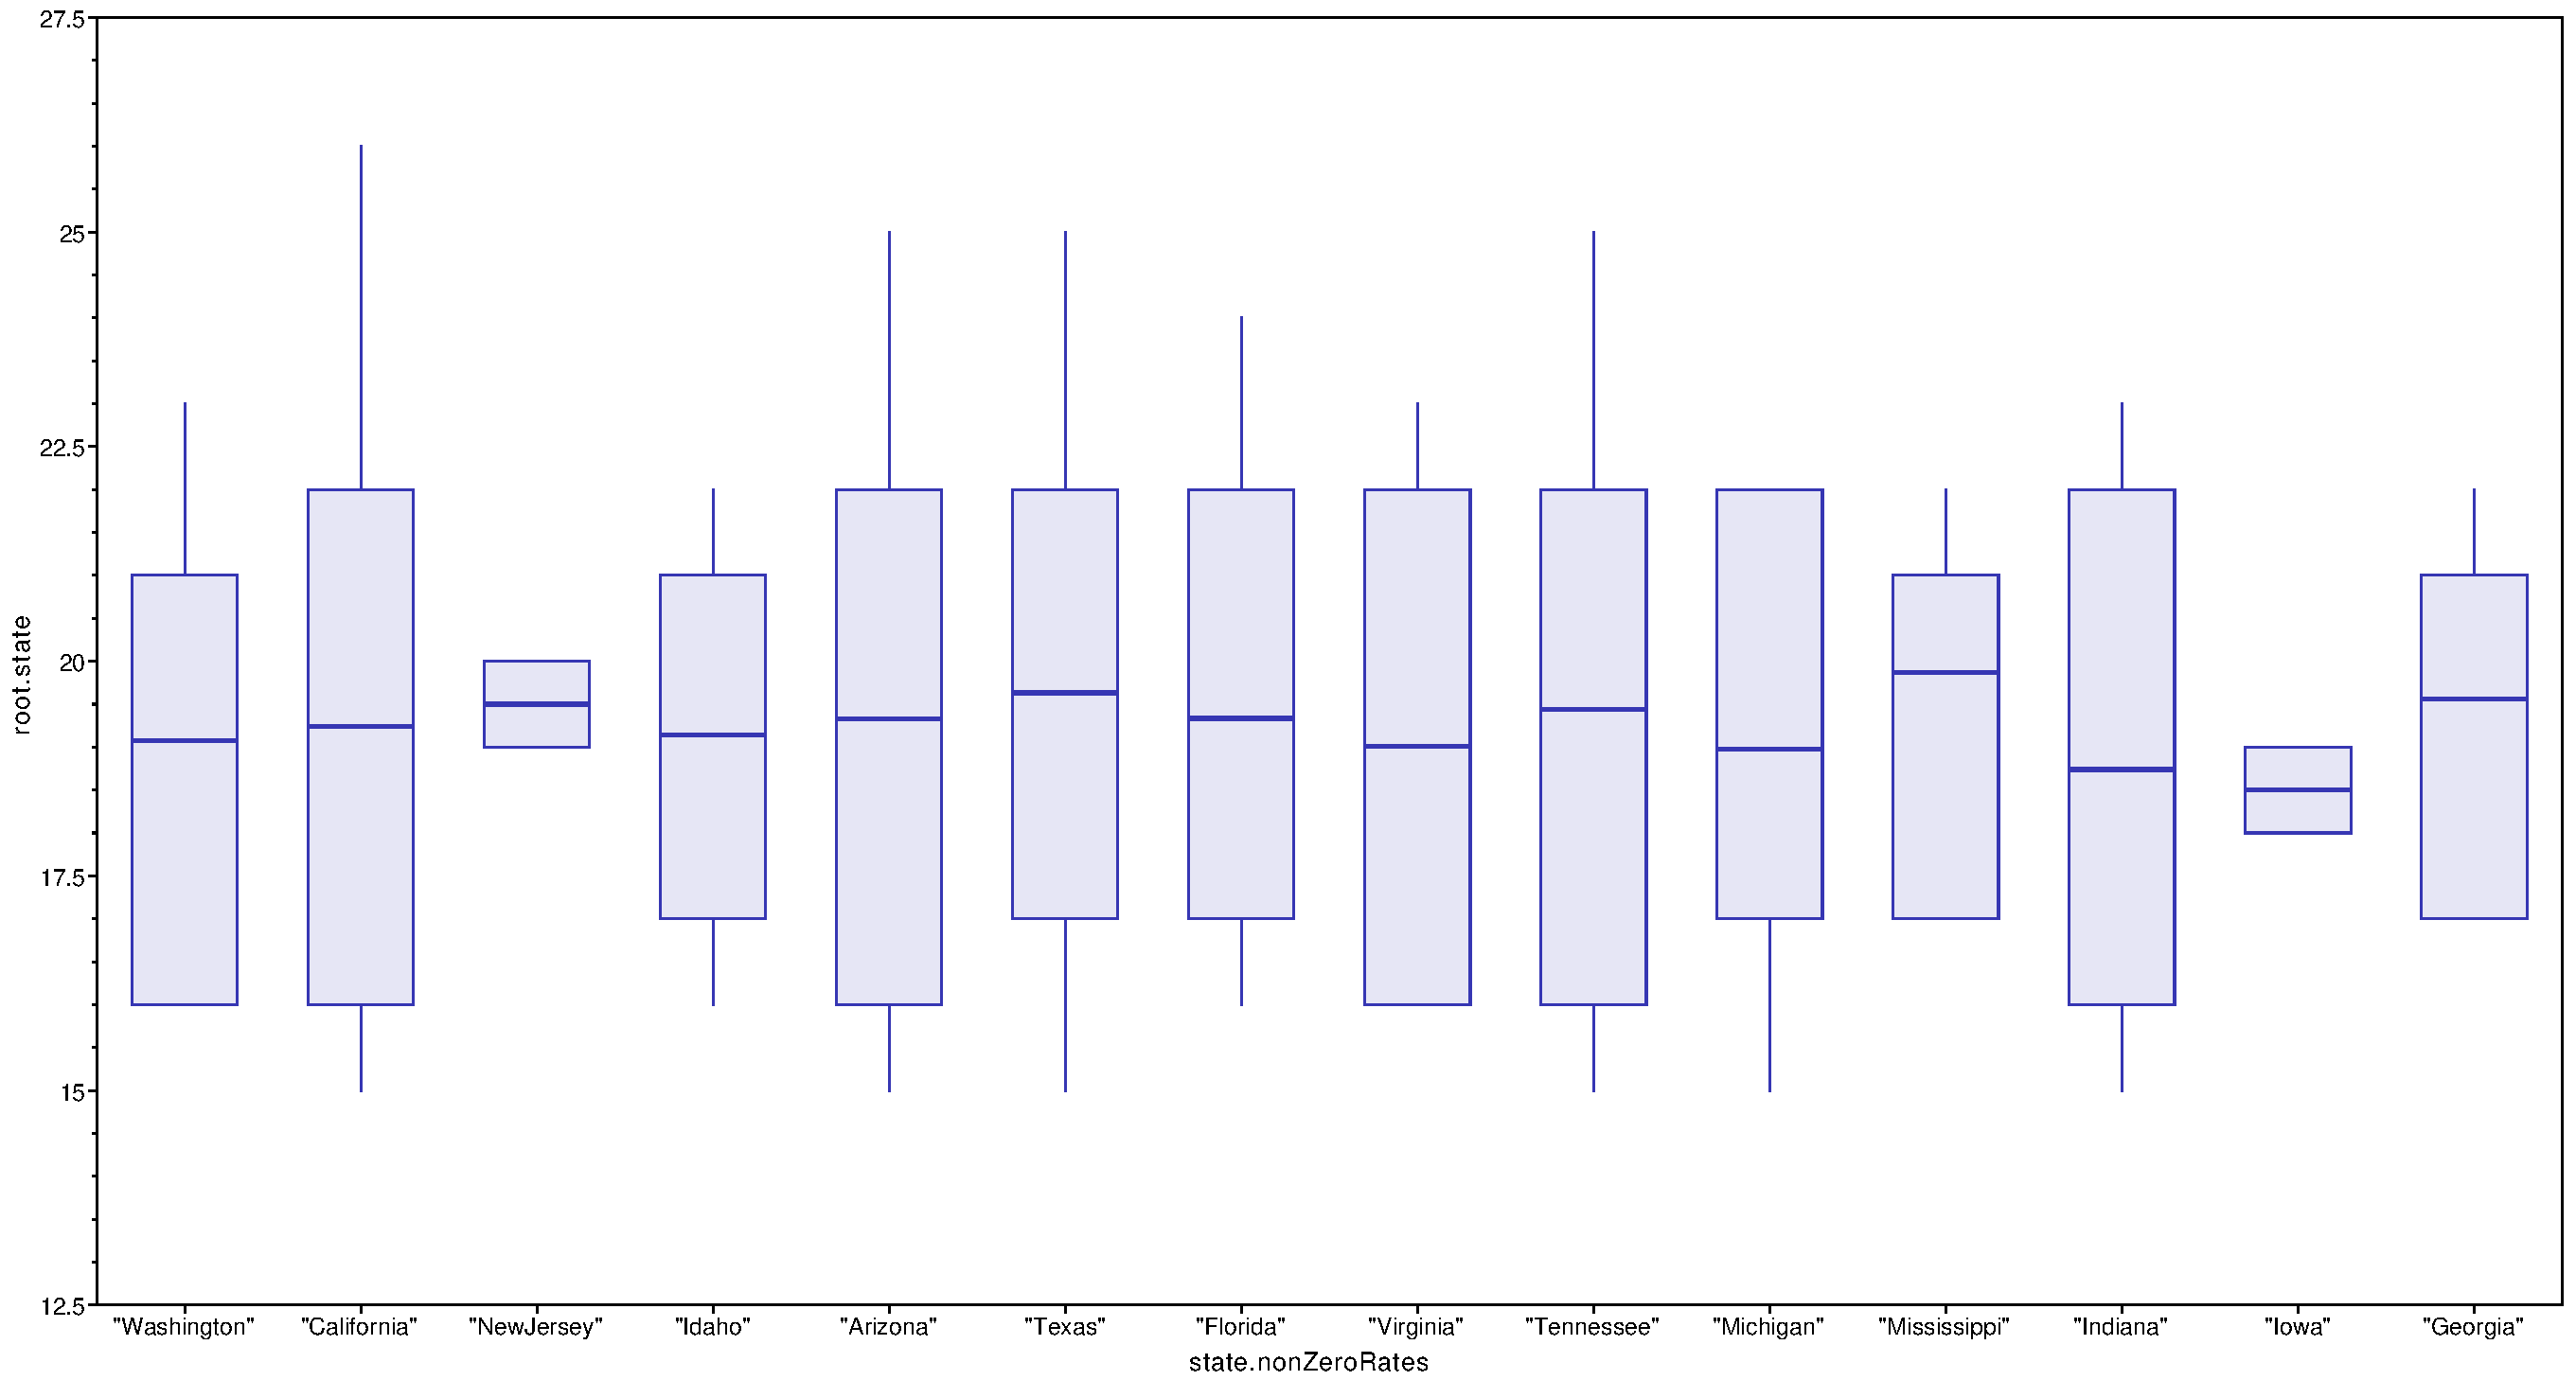
\includegraphics[width = .465\textwidth, height = 3cm]{./figures/rabv-catreal.pdf}}
\caption{Joint marginal and marginal density plots of: (a) two integer variables through a TangHuLu chart; (b) frequency plots the marginal density of multiple integer or categorical variables; (c) classic scatter or correlation plot for two continuous variables; (d) large correlation matrices for multiple ($> 2$) continuous variables.
%; (e) box-and-whisker plots for the joint marginal distribution of a continuous and an integer or categorical variable.
}
\label{fig:4tabs}
\end{figure}


Performing BSSVS in a discrete phylogeographic approach provides us with parameters of the integer and categorical trace type.
While a single parameter of such types can easily be visualised using a frequency plot, we have developed a TangHuLu chart to visualise the joint probability between two integer or categorical traces using coloured bubbles (see Figure \ref{fig:4tabs}:a).
The size of circle drawn is proportional to the joint probability, %the blue coloured circle is in the credible set of given a probability threshold default to 0.95, the red is in the set not in the credible set.
with the tile background being coloured if there is in fact a circle, to enhance visibility.
%The coloured background can also help to show the area of the credible set and non-credible set.
Multiple integer parameters can also be visualised using marginal density plots (see Figure \ref{fig:4tabs}:b), with a different colour scale being assigned to each parameter.
Both figures show a clear overlap in the number of non-zero transition rates in the discrete trait models for host and location, as identified using a BSSVS procedure.
The visualisation options for integer or categorical parameters are complemented with popular plots for continuous variables, such as a scatter or correlation plot (see Figure \ref{fig:4tabs}:c) for two continuous variables, which indicates a strong positive correlation between the clock rates of both discrete trait models.
We also provide an extension of such a scatter plot for multiple (i.e. more than two) continuous variables (see Figure \ref{fig:4tabs}:d; \citet{Murdoch}), which makes use of coloured ellipses to indicate the strength of correlation between each pair of continuous variables.
Colour gradients indicate the strength and direction of the correlation, with a colour gradient from white to dark blue indicating increasingly strong correlation and a colour gradient from white to dark red indicating increasingly strong anti-correlation.
Additionally, the strength of correlation is reflected in the shape of the ellipse drawn, with no correlation being drawn as a circle and perfect (anti-)correlation being drawn as a line.
%Finally, in order to display the joint marginal distribution between a continuous variable and an integer or categorical variable, we make use of box-and-whisker plots.
%Using such a plot (Figure \ref{fig:4tabs}:e), we can infer that the range of the non-zero transition rates can depend on the ancestral location state inferred at the root of the underlying phylogeny.

The Bayesian skygrid coalescent model \citep{gill2012improving} allows us to use Tracer to reconstruct the demographic history of RABV in North America by drawing the effective population sizes over time (see Figure \ref{fig:rabv}).
Given the properties of this coalescent prior, which requires to specify a grid of intervals over the timeframe of the epidemic, Tracer is able to infer this history without requiring a posterior sample of trees.
According to Tracer's skygrid plot, it is clear that rabies virus has successfully established itself in North American bat species, with its numbers rising steadily throughout recent centuries.
Following a decline in numbers at the end of last century, we observe a recent sharp increase in population size of RABV in North American bats.


\begin{figure}[ht]
\centerline{
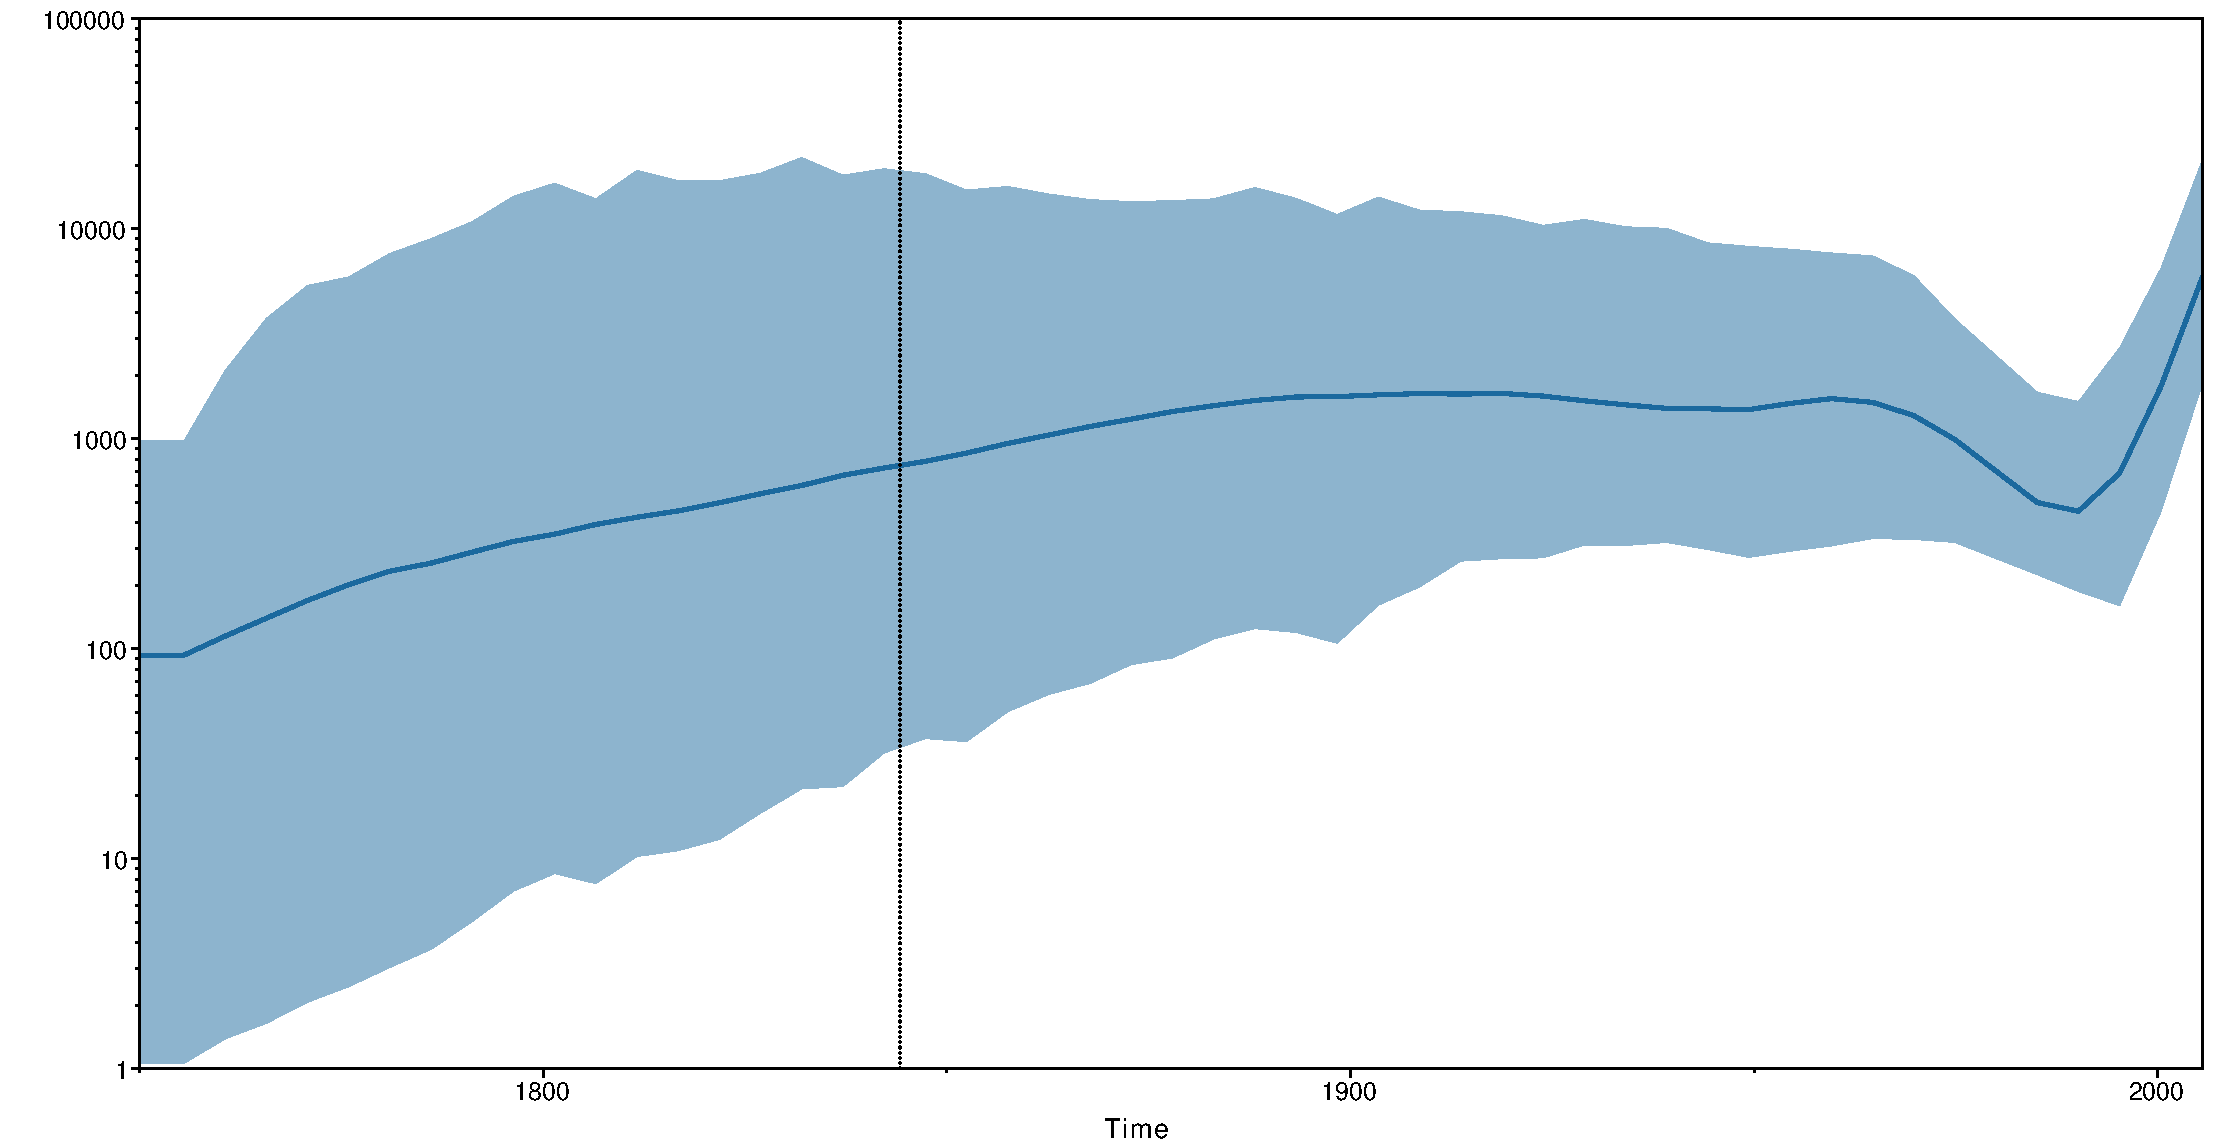
\includegraphics[width=0.46\textwidth]{./figures/rabv-skygrid.pdf}
}
\caption{Estimating the effective population sizes over time using a Bayesian skygrid demographic reconstruction for rabies virus in North America.}
\label{fig:rabv}
\end{figure}



\section*{Availability}

Tracer 1.7 is open-source under the GNU lesser general public license and available in both executable and source code forms at \url{http://beast.community/tracer}.
It requires Java version 1.6 or greater.
Github houses the Tracer's source code within \url{https://github.com/beast-dev/tracer}, and links to a GoogleGroup discussion group related to Tracer, i.e. the ``beast-users" group (\url{http://groups.google.com/group/beast-users}).
This page also links to a sizeable list of self-contained, step-by-step tutorials covering basic to advance usage of Tracer to summarise posterior distributions of a large set of phylogenetic models simulated using BEAST.
For example, popular tutorials describe how to use Tracer to generate marginal parameter summaries and infer population dynamics trajectories over time.



%\section*{Old Text}
%
%%You can also select the "Demographic Analysis" from the Analysis menu - This plots the distribution of demographic population sizes over time for a number of models (constant size, exponential growth \& logistic growth) that are available in BEAST. This involves you selecting the traces for each parameter of the model. You should only select the model that was actually run under BEAST (e.g., if you ran an exponential growth model, you shouldn't plot the constant population size model).
%
%%The "Analysis" menu also contains options for performing Bayesian Skyline reconstructions and for calculating Bayes Factors between runs.
%
%Feature list:
%\begin{itemize}
%\item KDEs
%\item cheap marginal likelihood estimators
%\item demographic trajectory reconstruction
%\end{itemize}
%
%%Model selection HME and AICM have been removed
%New features:
%\begin{itemize}
%\item Three trace types: real, integer, string
%\item Kernel density estimates
%\item Conditional posterior distribution
%%\item HME
%%\item AICM
%\end{itemize}
%
%%\begin{figure}[H]
%%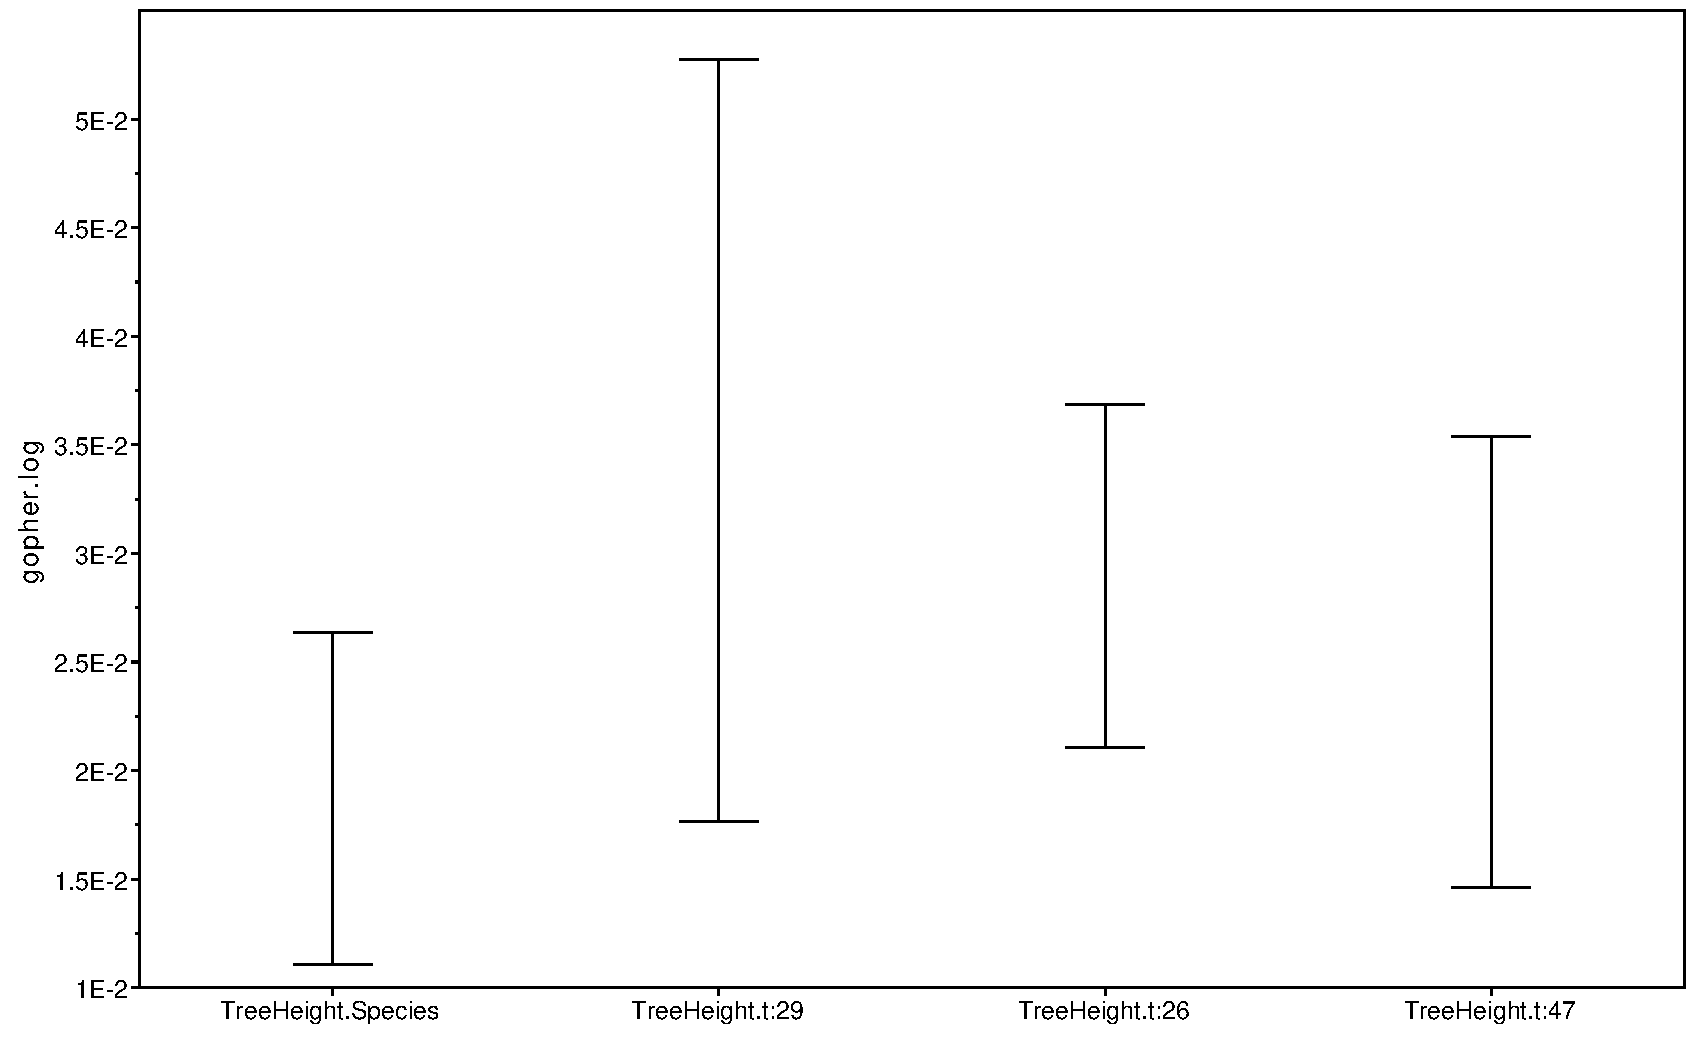
\includegraphics[width=.5\textwidth]{./figures/comp-95HPD.pdf}
%%\caption{The comparison of  95\% HPD intervals from multi-trace}
%%\label{fig:comp95HPD}
%%\end{figure}
%
%%\begin{figure}[H]
%%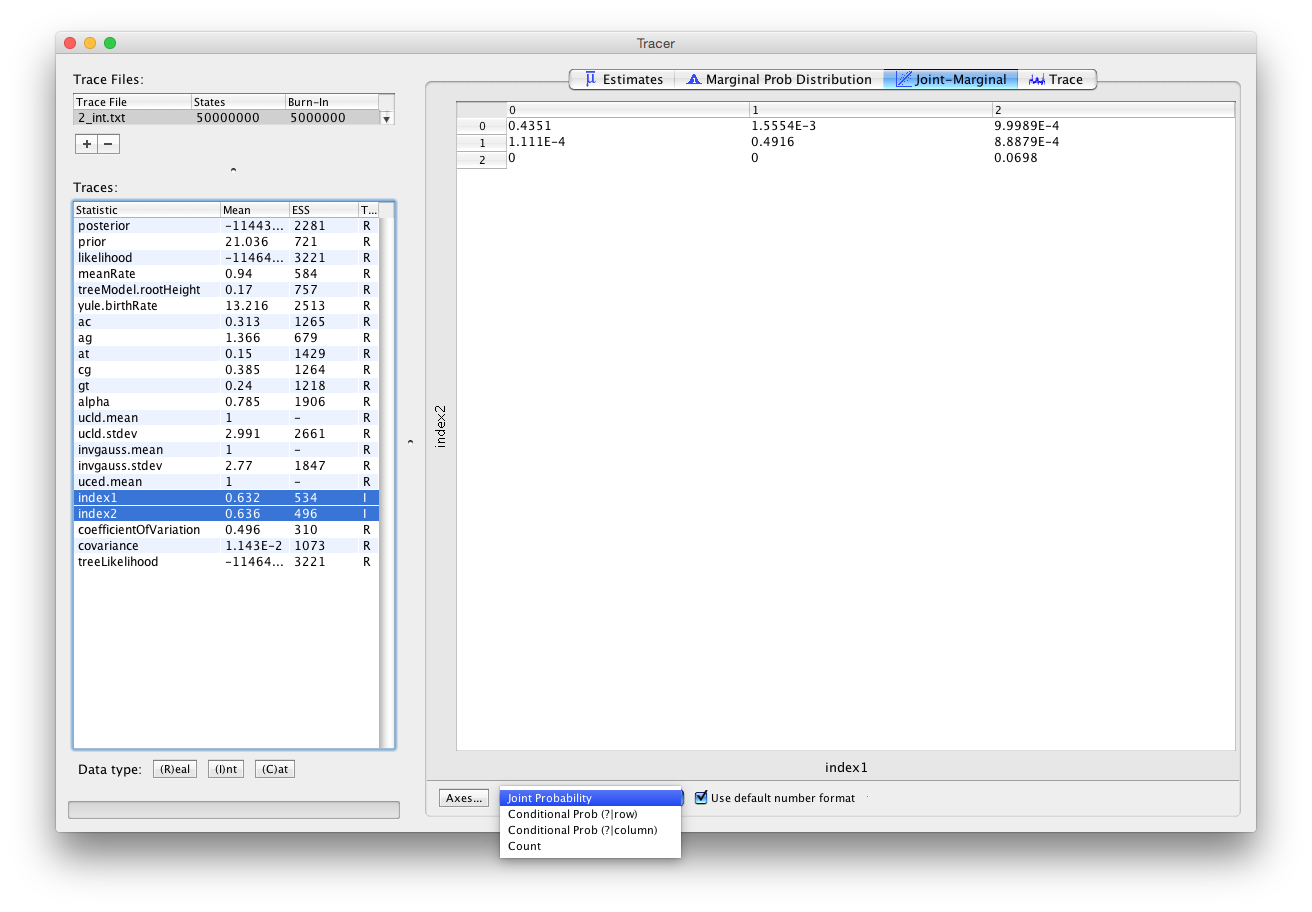
\includegraphics[width=.5\textwidth]{./figures/jointPrInt.png}
%%\caption{The Joint probability table of two integer traces}
%%\label{fig:int:jointpr}
%%\end{figure}
%
%%\begin{figure}[ht]
%%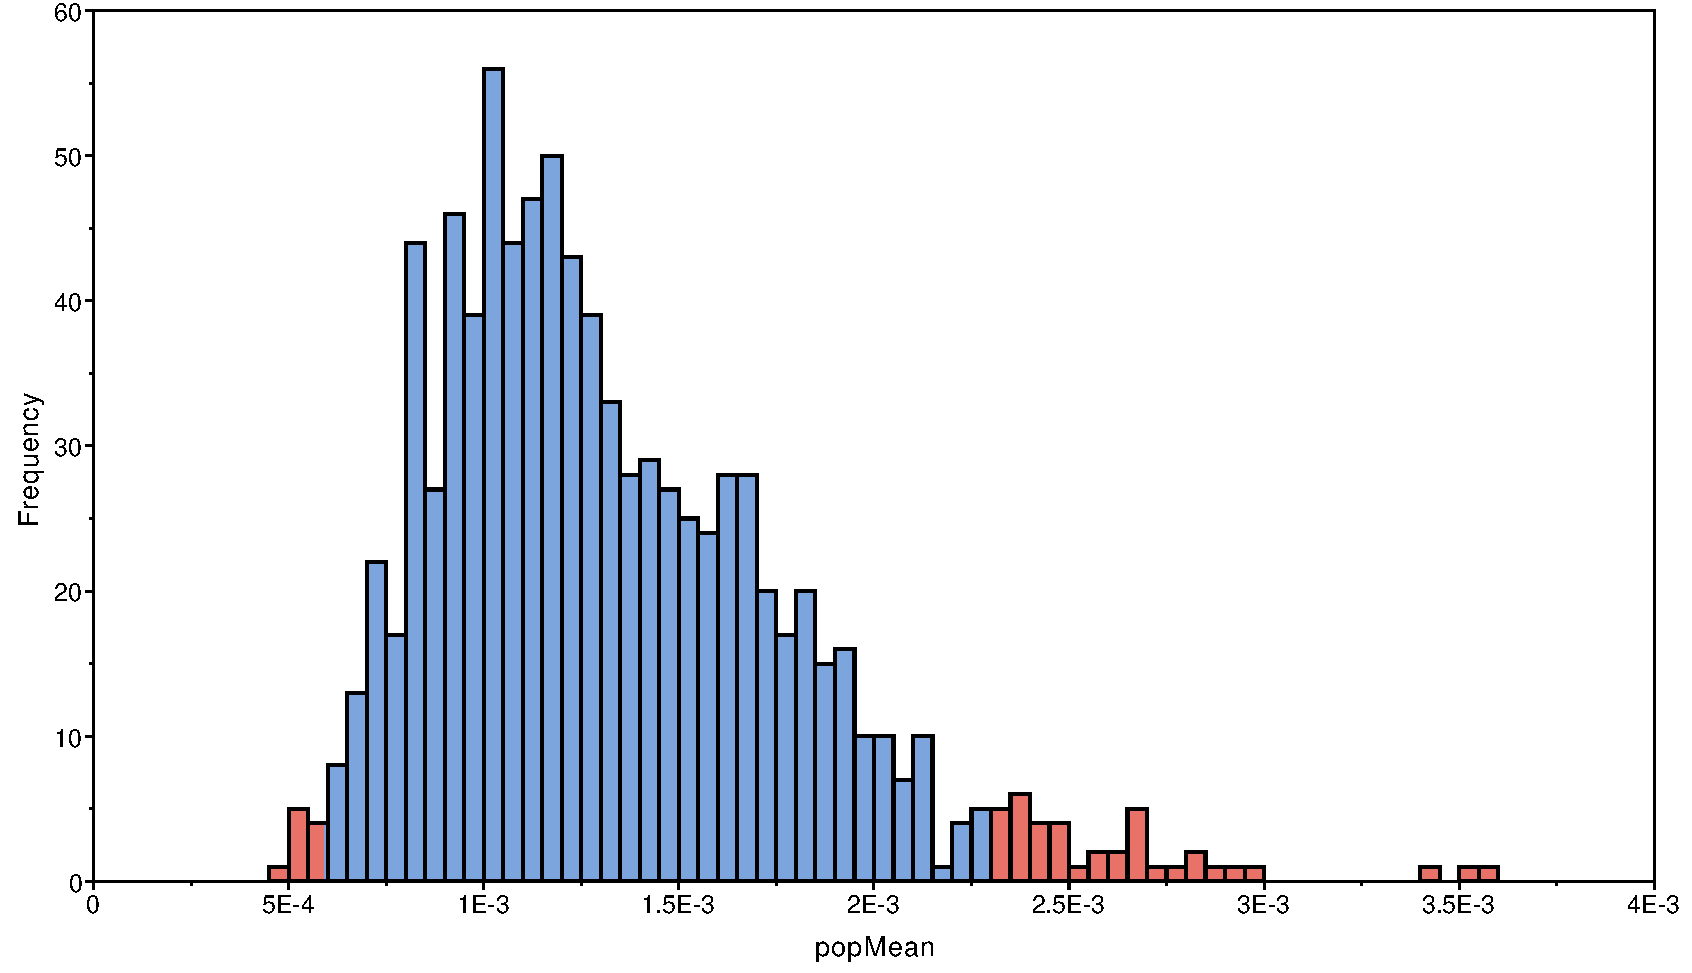
\includegraphics[width=.5\textwidth]{./figures/frequency.pdf}
%%\caption{A frequency distribution for a continuous trace}
%%\label{fig:freq}
%%\end{figure}
%%\begin{figure}[ht]
%%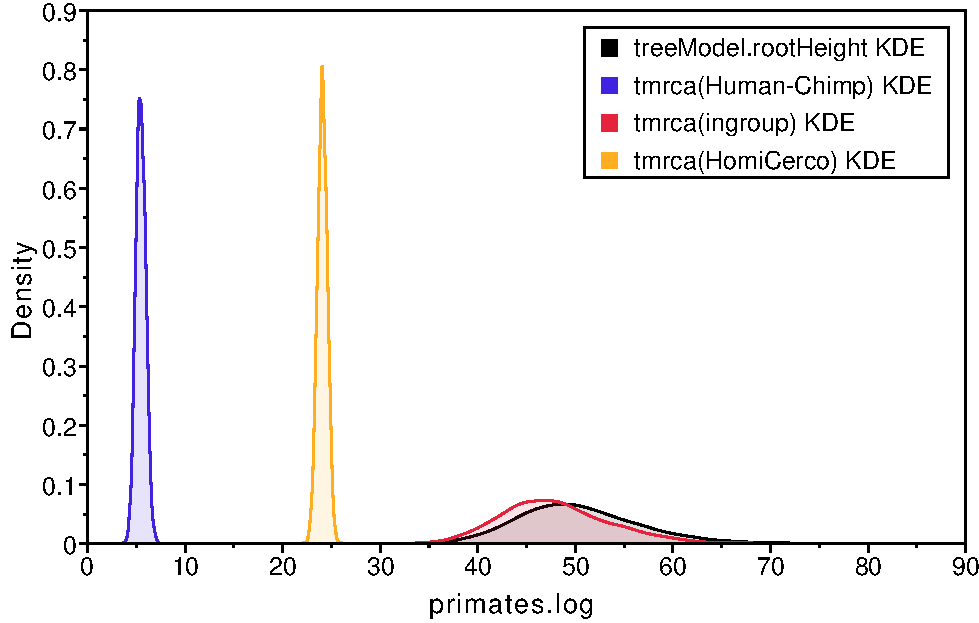
\includegraphics[width=.5\textwidth]{./figures/multiKDE.pdf}
%%\caption{KDE of multiple traces}
%%\label{fig:multiKDE}
%%\end{figure}
%%\begin{figure}[ht]
%%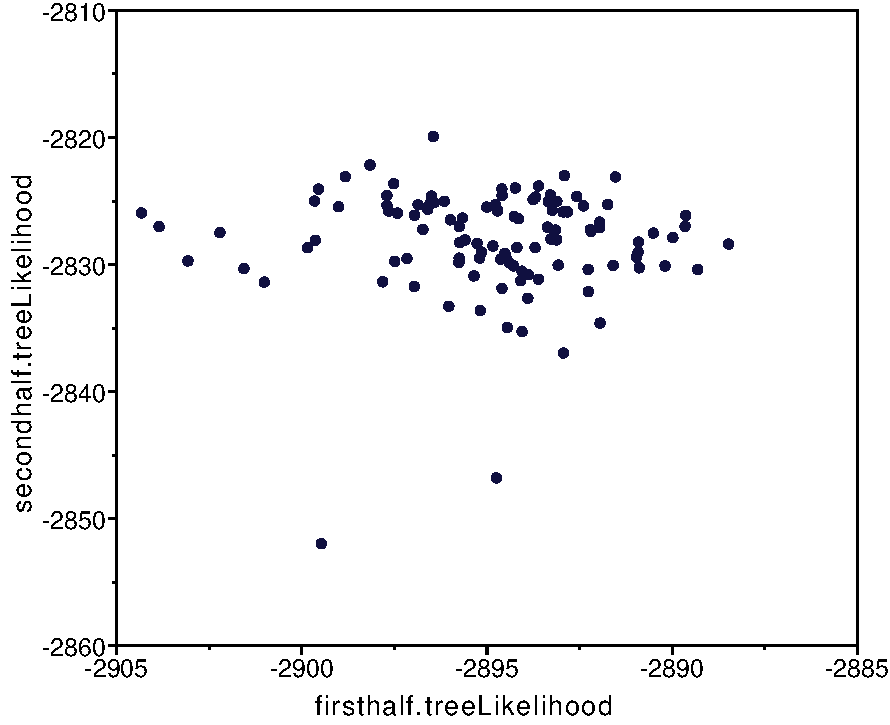
\includegraphics[width=.5\textwidth]{./figures/joint-marginal.pdf}
%%\caption{The joint-marginal distribution of two selected tes}
%%\label{fig:trace}
%%\end{figure}
%%\begin{figure}[ht]
%%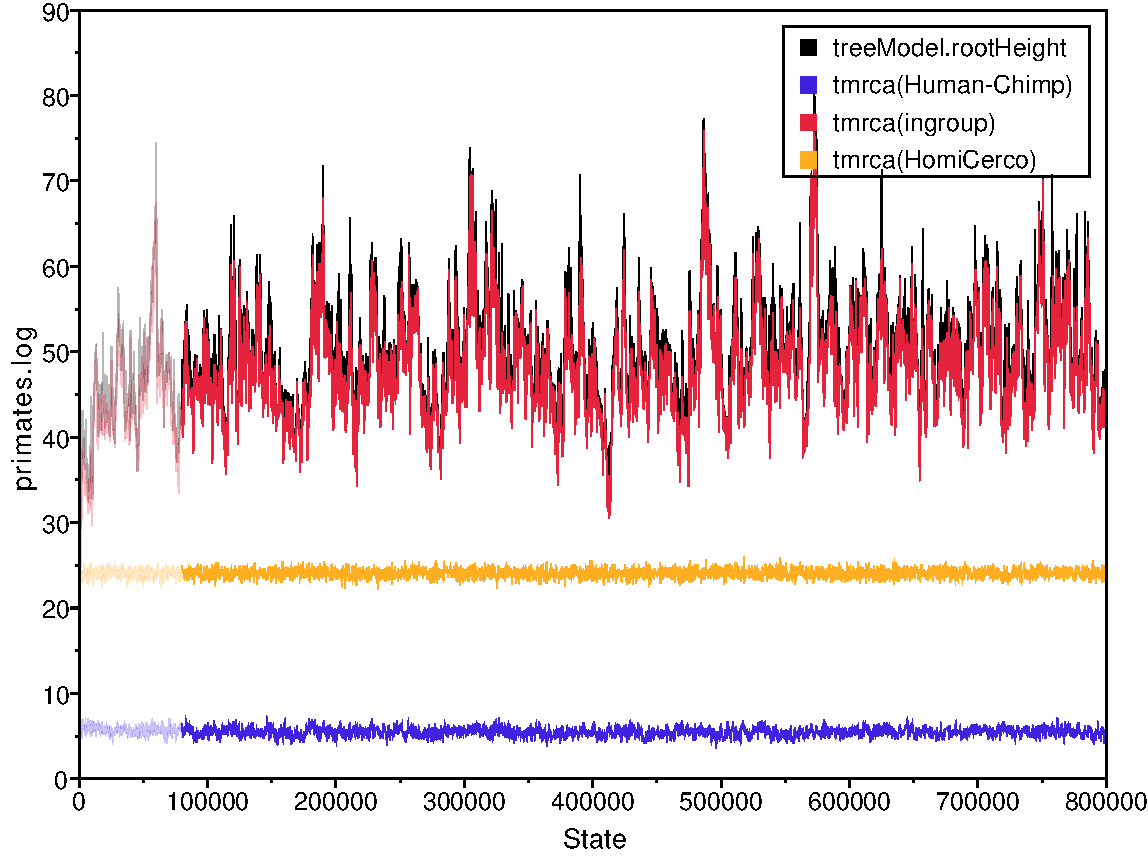
\includegraphics[width=.5\textwidth]{./figures/trace.pdf}
%%\caption{The selected traces against state}
%%\label{fig:trace}
%%\end{figure}
%
%
%\subsubsection*{Diagnostics:} Blah blah
%
%\subsubsection*{Demographic reconstruction:}
%
%%\subsubsection*{Model selection:}
%
%\subsubsection*{Conditional posterior distribution:}

%Fairly general solution to looking at conditional posterior distributions;

%Specifically, support for BSSVS forms of model averaging, in which some parameters are only in the likelihood when their submodel is "indicated" by some indicator function that is usually a discrete, integer or boolean variable. In that case the posterior of the parameter should not include the states when it was sampled only in the prior because the submodel it belonged to was "turned off". This is relevant for EBSP, Random Local Clocks model, microsatellite model averaging and relaxed clock model averaging methods all from my group in last couple of years. Also relevant for BSSVS in phylogeography as well depending on how the state is logged.
%\section*{Taken from the Tracer website}

%Tracer is a program for analysing the trace files generated by Bayesian MCMC runs (that is, the continuous parameter values sampled from the chain). It can be used to analyse runs of BEAST \citep{drummond2012bayesian,drummond2012bayesian}, BEAST2 \citep{bouckaert2014beast2}, MrBayes \citep{ronquist2012mrbayes}, RevBayes \citep{hohna2016revbayes}, LAMARC \citep{kuhner2006lamarc}, Migrate \citep{beerli2006comparison} and possibly other MCMC programs.

%Although Tracer can be used with programs other than BEAST, users may find it useful to join the BEAST users mailing list. This is used to announce new versions and advise users about bugs and problems.

%You can join the mailing list here:
%http://groups.google.com/group/beast-users

%The website for BEAST (and Tracer) is here:
%http://beast.bio.ed.ac.uk/

%At present there is no detailed manual for this application, you will simply have to play around and see what happens. Basically you can select the trace file in the top left of the window, the individual parameter in the bottom left and the analysis appears on the right.

%There are 4 analysis tabs to choose from:

%Estimates - this shows the mean, stdev, confidence intervals and other statistics about the selected parameter. A frequency distribution will also be plotted.
%Density - this shows the Bayesian posterior density plot for the selected parameter.
%Joint-Marginal - this only appears if exactly 2 parameters are chosen (hold down shift to select multiple parameters). It then plots one against the other to look at their joint-marginal distribution.
%Trace - this shows the trace of the parameter against state or generation number. Use this to check mixing, choose a suitable burn-in and look for trends that might suggest problems with convergence.
%Multiple parameters can be selected by holding down the shift key. This will overlay the plots for the different parameters allowing comparisons to be made. You can also select multiple trace files as well to compare different runs. If multiple trace files have the same trace names then a "Combined" trace will automatically appear. This can be selected as well as the individual trace files.

%You can also select the "Demographic Analysis" from the Analysis menu - This plots the distribution of demographic population sizes over time for a number of models (constant size, exponential growth \& logistic growth) that are available in BEAST. This involves you selecting the traces for each parameter of the model. You should only select the model that was actually run under BEAST (e.g., if you ran an exponential growth model, you shouldn't plot the constant population size model).

%The "Analysis" menu also contains options for performing Bayesian Skyline reconstructions and for calculating Bayes Factors between runs.

%The "Print" function in the "File" menu will print the current graph or table and the "Export Data" function can be used to export the data from the plots for use in another graphic package.

%To export the currently displayed graphic use the "Export PDF" function in the "File" menu.


\section*{Acknowledgements}

This work was supported in part by the Wellcome Trust through project 206298/Z/17/Z (Artic Network), the European Union Seventh Framework Programme under grant agreement no. 725422-RESERVOIRDOCS, the National Science Foundation through grant DMS 1264153, the National Institutes of Health under grant R01 AI107034, and the Marsden Trust.
GB acknowledges support from the Interne Fondsen KU Leuven / Internal Funds KU Leuven.


%\section*{References}
% The bibtex filename
\bibliographystyle{natbib}
\bibliography{tracer17}

\end{document}

